%% Peaks in the MAP or in SIGNAL-TO-NOISE ???

%% Back up statements about completeness / purity -- more details
%% about multiple SED tests.


%% Matched filter:

% DAOphot source detection ("find") uses a type of matched filter. It's been fairly successful.
% FOCAS
% Palomar Distant Cluster Survey (Postman et al 1995)

% Catalog extraction in SZ cluster surveys: a matched filter approach
% http://www.aanda.org/articles/aa/full/2006/44/aa5034-06/footnode.html

% An automated cluster finder: the adaptive matched filter
% http://iopscience.iop.org/0004-637X/517/1/78

% Matched filter source detection applied to the rosat pspc and the determination of the number-flux relation
% http://adsabs.harvard.edu/full/1995apj...451..542v

% Observational limits on terrestrial-sized inner planets around the CM Draconis system using the photometric transit method with a matched-filter algorithm
% http://iopscience.iop.org/0004-637X/535/1/338

% Galaxy clusters in the CFHTLS-First matched filter candidate catalogue of the Deep fields
% http://www.aanda.org/articles/aa/abs/2007/01/aa6088-06/aa6088-06.html


%% TODOs: 
%% --add polemic about misuse of the word ``optimal'' in astronomy --
%%   the way it is most commonly misused, the word ``good'' should be
%%   used instead -- ``we found some parameter settings that seem
%%   optimal'', or ``this is more optimal than that''.  ONE THING CAN'T
%%   BE *MORE* OPTIMAL THAN ANOTHER.  It's either optimal or it isn't.
%%   Be sure to say that we actually do mean optimal, in that we define
%%   a metric and then define a procedure that produces the biggest
%%   possible value under that metric.

%% --for ``bandpass filter'' we're really talking about the whole
%%   system throughput -- including CCD sensitivity and not just the
%%   filter per se.

%% --need to talk about *thresholds*, relate to false-positive rate,
%%   and admit that by running more filters we will produce more false
%%   positives.

% - number of peaks in a Gaussian field

% -''worser''

% -Discussion: natural extensions to deal with point-spread function, noise-model, calibration, and time-domain uncertainties.

% -Intro: pixels or regions --- actually ``regions'' is another notion I'd like to dispel.

% -optimal linear detection: need to say a little more about PSF
% correlation if we're really going to push all the content to the
% appendix!  We're fairly mathy up to this point.  Also need to repeat
% the punch line, to introduce notation if nothing else.

%  Szalay et al. 1999 AJ, 117, 68, often referred to as the "chi squared" method.

\documentclass[letterpaper,preprint]{aastex}
\usepackage{bm}
\usepackage{calc}
\usepackage{amssymb, amsmath}
\usepackage{hyperref}
\newcounter{address}
\newcommand{\doctype}{paper}
\newcommand{\equationname}{equation}
\newcommand{\eqnref}[1]{\mbox{\equationname~\ref{#1}}}
\newcommand{\appref}[1]{\mbox{Appendix~\ref{#1}}}
\newcommand{\Appref}[1]{\mbox{Appendix~\ref{#1}}}
\newcommand{\tabref}[1]{\mbox{Table~\ref{#1}}}

\newcommand{\niceurl}[1]{\mbox{\href{#1}{\textsl{#1}}}}

\newcommand{\latin}[1]{\emph{#1}}
\newcommand{\etal}{\latin{et\,al.}}
\newcommand{\ie}{\latin{i.e.}}
\newcommand{\apriori}{\latin{a priori}}
\newcommand{\USNOB}{USNO-B Catalog}
\newcommand{\an}{\textsl{Astrometry.net}}
\newcommand{\sn}{{[s/n]}}
\newcommand{\sntotal}{\sn_{\mathrm{total}}}
\newcommand{\fwhm}{{\theta_{\mathrm{FWHM}}}}
\newcommand{\RA}{{\mathrm{RA}}}
\newcommand{\Dec}{{\mathrm{Dec}}}
\newcommand{\vecmu}{\bm{\vec{\mu}}}
\newcommand{\mualpha}{{\mu_\alpha}}
\newcommand{\mudelta}{{\mu_\delta}}
\newcommand{\var}[1]{\mathrm{Var}({#1})}
\newcommand{\unit}[1]{\mathrm{#1}}
\renewcommand{\mag}{\unit{mag}}
\newcommand{\s}{\unit{s}}
\newcommand{\yr}{\unit{yr}}
\newcommand{\km}{\unit{km}}
\newcommand{\pc}{\unit{pc}}
\newcommand{\kpc}{\unit{kpc}}
\newcommand{\mas}{\unit{mas}}
\newcommand{\pix}{\unit{pix}}
\newcommand{\kmpers}{\km\,\s^{-1}}
\newcommand{\masperyr}{\mas\,\yr^{-1}}
\renewcommand{\arcsec}{\unit{arcsec}}
\newcommand{\arcsecperyr}{\arcsec\,\yr^{-1}}
\newcommand{\code}[1]{\texttt{#1}}
\newcommand{\mean}[1]{\left<{#1}\right>}

\renewcommand{\thefootnote}{\fnsymbol{footnote}}

\newcommand{\figpart}[1]{\textbf{#1}}
\newcommand{\fig}{Figure}
\newcommand{\figref}[1]{\mbox{\fig~\ref{#1}}}
\newcommand{\detmap}{detection map}
\newcommand{\Detmap}{Detection map}
\newcommand{\fluxmap}{flux map}
\newcommand{\fmap}{F}
\newcommand{\drawnfrom}{\sim}
\newcommand{\gaussianN}{\mathcal{N}}
\newcommand{\gaussian}[1]{\gaussianN\!\left(#1\right)}
\newcommand{\gaussx}[1]{\hat{\gaussianN}\!\left(#1\right)}
%\newcommand{\gaussx}[1]{\mathfrak{N}\!\left(#1\right)}
%\newcommand{\psf}{\mathrm{psf}}
\newcommand{\psf}{\psi}
\newcommand{\psfat}[1]{\psf_{#1}}
\newcommand{\psfnorm}{\norm{\bm{\psf}}}

\newcommand{\signoise}{[S/N]}
\newcommand{\snr}[1]{\mathbb{SN}(#1)}
%\newcommand{\snr}[1]{\mathcal{SN}(#1)}

\newcommand{\norm}[1]{\left\lVert #1 \right\rVert}
\newcommand{\expect}[1]{\left\langle #1 \right\rangle}
\renewcommand{\var}[1]{\mathrm{var}\left( #1 \right)}
\newcommand{\sky}{\mathrm{sky}}
\newcommand{\psfw}{w}
\newcommand{\dd}{\mathrm{d}}
\newcommand{\noise}{e}
\renewcommand{\vec}[1]{\boldsymbol{#1}}
\newcommand{\thetavec}{\vec{\theta}}
\newcommand{\avec}{\vec{a}}
\newcommand{\ivec}{\vec{i}}
\newcommand{\jvec}{\vec{j}}
\newcommand{\kvec}{\vec{k}}
\newcommand{\cvec}{\vec{c}}
\newcommand{\posvec}{\vec{x}}
\newcommand{\coord}[2]{(#1, #2)}
\newcommand{\iina}{\ivec \,\, \mathrm{in} \,\, \mathcal{A}}

\newcommand{\commentout}[1]{}

\slugcomment{Submitted to The Astronomical Journal}

\begin{document}
\title{Principled point-source detection in collections of astronomical images}
\author{%
  Dustin Lang\altaffilmark{1,2,3},
  David W. Hogg\altaffilmark{4,5},
  \& Others}

\altaffiltext{1}{To whom correspondence should be addressed; \texttt{dstndstn@gmail.com}}
\altaffiltext{2}%
{Department of Astronomy \& Astrophysics and Dunlap Institute,
  University of Toronto,
  50 Saint George Street, Toronto, ON, M5S 3H4, Canada}
\altaffiltext{3}%
{Department of Physics \& Astronomy,
  University of Waterloo,
  200 University Avenue West,
  Waterloo, ON, N2L 3G1, Canada}
\altaffiltext{4}{Center for Cosmology and Particle Physics, Department of Physics, New York University, 4 Washington Place, New York, NY 10003, USA}
\altaffiltext{5}{Max-Planck-Institut f\"ur Astronomie, K\"onigstuhl 17, D-69117 Heidelberg, Germany}

\begin{abstract}
  Given a collection of astronomical images of the same patch of sky, it is
  possible to detect sources fainter than those detectable in any
  individual image.
  %
  In some traditional astronomical image analysis codes, this
  operation is performed by first co-adding the images (after
  interpolation to a common grid), and running standard image-reduction
  routines on the co-added image.
  %
  This approach fails to make use of all the available information in
  the images when the images contain different levels of noise, have
  different point-spread functions, or are taken through different
  wavelength bandpasses.
  % 
  Here we show that---under stated assumptions---optimal point-source
  detection proceeds by an operation that looks very much like
  convolution, interpolation, and co-addition, but which does
  \emph{not} produce a final image that is a sensible measure of the
  intensity field; it is instead a heterogeneous significance map.
  %
  We
  then show how to detect sources in images taken through different
  bandpass filters by combining these significance maps.  This
  requires prior information about the distribution of spectral energy
  distributions.  We show how traditional approaches can be
  interpreted as assuming particular spectral energy distribution
  priors.  After sources have been detected in the way
  outlined here, photometry, astrometry, and other measurements should
  be made by simultaneously fitting models to the collection of pixels
  in the non-co-added individual images (which have not been degraded
  by convolution, interpolation, or co-addition).  We show that the
  best practices differ from common practices only in small ways; in
  particular, best practices are not computationally expensive.
\end{abstract}

\keywords{
    methods:~statistical ---
    techniques:~image~processing
}

\section{Introduction}

There are few operations in astronomy more important than the
detection of stars or point sources.
Indeed, many astronomical discoveries come down to point-source
detection.
What is the best method for performing such detection?
Here we answer that question, in the limited context of isolated
sources, uniform sky-limited noise, and well-understood point-spread
function.
Even in this limited context, the subject is rich and valuable; more
general---and more difficult---cases will be illuminated if we can
understand the simplest case first.

Fundamentally, when much is understood about a signal latent in noisy
data, the best detection methods are (or look like) \emph{matched
filters}.
A matched filter is a model of the expected signal with which the data
are \emph{cross-correlated}. % (often wrongly called ``convolved'').
Peaks in the cross-correlation are candidate signal detections.
In astronomical point-source detection, the expected signal is the
point-spread function (PSF), and the cross-correlation operation is often
wrongly called ``convolution''.
Matched filters are well used in astronomy, in contexts ranging from
spectroscopy (CITE) to galaxy cluster detection \citep{postman},
ultra-faint galaxies \citep{willman} and gravitational
radiation (CITE).


In what follows, we will argue for matched filtering for point-source
detection.
This is not new (CITE); what is new is that we consider the common
context of heterogeneous (in point-spread function and sensitivity)
multi-epoch, multi-band imaging.
A key idea is that when the imaging is multi-band, the expected
spectral-energy distribution (spectrum) of the source becomes part of
the matched filter.
Any method that attempts to detect sources in multi-band
imaging---even if it does so independently in the different bands---is
effectively making implicit assumptions about spectral-energy
distributions.
The wronger these assumptions, the worser the source detections.

In the Real World, astronomers never precisely know their point-spread
function, their noise model, their flat-field (or other calibration
parameters), nor the spectral-energy distributions of the sources of
greatest interest.
Also, often, the sources of interest aren't point sources or perhaps
vary with time.
In these cases, we advocate parameterizing ignorance, and operating
with the union of all possibly appropriate matched filters.
We will fully execute this idea here when it comes to spectral-energy
distributions, but there are natural extensions to deal with
point-spread function, noise-model, calibration, and time-domain
uncertainties.


Often, astronomers ``co-add'' their imaging to find faint objects.
Technically, this step is only justifiable if the bandpass and
point-spread function are the same for all images, and the images
ought to be weighted according to sensitivity.
Co-addition is not necessary for source detection, of course; it is
possible to combine low-significance source-detection information
coming from many images and do as well or better than co-addition.
An amusing conclusion of this project is that in the principled limit,
the combination of source-detection information looks very much like a
(weighted) co-addition of (smoothed) data!

That is, in what follows, we will detect sources as above-threshold
pixels in a weighted co-add of PSF-correlated input images.
We will call this object a ``detection map''.
This detection map is the best thing to use for source detection.
Once sources are detected, of course, the detection map should be put
aside, and source properties (positions, colors, and so on) ought to
be measured (inferred) from the raw pixels in the collection of input
images via a likelihood function.
That measurement and likelihood function is beyond the scope of this
paper, but the subject of a parallel research program (CITE).

\section{Our image model}

We consider idealized astronomical images such as those obtained from
a CCD in broadband optical imaging.
%
We will assume that the image is well calibrated: the flat-field or
per-pixel sensitivities are known, as is the astrometric calibration
and the point-spread function.
%
We assume the image pixels contain additive, independent, Gaussian
noise.  This is reasonable for images with significant background or
``sky'' noise and read noise, where the mean sky level has been
estimated and subtracted.  (Background flux is typically Poisson
distributed, which at high count levels is well approximated by the
Gaussian.)
%

Importantly, we will assume the PSF function $\psi(\cdot)$ is the
pixel-convolved PSF, not simply the PSF due to optics and atmosphere,
so image pixels are a sampling and not a convolution or binning of the
PSF-convolved intensity field.
We will assume the PSF is well-sampled by the pixels.

\section{Detecting a point source in a single image}

In this section, we will assume that the (perhaps tiny) image of
interest contains only a single isolated point source $k$ with some
constant unknown flux $F_k$ and position $\kvec$ in pixel coordinates.

As described above, we will assume any background level has been
estimated perfectly and subtracted, so that the image pixels contain
only signal due to the source plus zero-mean, pixelwise-independent,
Gaussian noise of known variance;
\begin{eqnarray}\displaystyle
  C_{\jvec} &=& F_k \, \psi(\jvec - \kvec)  + \noise_{\jvec} \quad ,
\end{eqnarray}
where $C_{\jvec}$ is the image pixel value in pixel $\jvec$ (a
two-dimensional index), $F_k$ is the scalar flux of the source,
$\psi(\cdot)$ is the point-spread function, and $\noise_{\jvec}$ is
the noise term.  We can also write this as
\begin{eqnarray}\displaystyle
  C_{\jvec} &\drawnfrom& \gaussx{F_k \, \psi(\jvec - \kvec), \sigma_1^2}
\label{eq:modelimg}
\end{eqnarray}
where the symbol ``$\drawnfrom$'' means ``drawn from the
distribution'', and $\gaussx{\mu,\sigma^2}$ is the Gaussian
distribution with mean $\mu$ and variance $\sigma^2$; $\sigma_1^2$ is
the variance of the per-pixel noise values $\noise_{\jvec}$, assumed
constant in this section.







\subsection{Optimal linear detection}

In \appref{app:lindet}\ we show that \emph{correlating} an image by
its PSF results in an optimal detector for isolated point sources.

We define the \emph{\detmap} $D_{\jvec}$ as the correlation of
the image with its PSF model, scaled to be in convenient units:
\begin{equation}
D_{\jvec} = \frac{1}{\psfnorm^2} \sum_{\iina} \psfat{\ivec} \, S_{\ivec + \jvec} \quad ,
\label{eq:detmap}
\end{equation}
where $\mathcal{A}$ is the support of the PSF and
$\psfat{\ivec} = \psf(\ivec)$ is an image of the PSF evaluated at
integer-offset pixel positions $\ivec$.  The PSF norm $\psfnorm$ is
\begin{equation}
\psfnorm = \sqrt{\sum_{\iina} \psfat{\ivec}^2} \quad ,
\end{equation}
and as shown in \appref{app:gaussnorm}, a Gaussian PSF with standard
devation $\psfw$ pixels has a norm approximately:
\begin{equation}
  \norm{\bm{\psf^G}} \simeq \frac{1}{2 \sqrt{\pi} \psfw} \quad .
\end{equation}
The per-pixel error in the \detmap\ is given by
\begin{equation}
\sigma_{D} = \frac{\sigma_1}{\psfnorm} \quad .
\end{equation}


We have scaled the \detmap\ so that each pixel contains the
maximum-likelihood total counts of a source centered at that pixel.
That is, computing at pixel $\jvec$ the total source counts
$C^{\ast}_{\jvec}$ to minimizes the chi-squared ($\chi^2$) residual
within the support of the PSF:
\begin{equation}
  C^{\ast}_{\jvec} = \arg\min_{c} \sum_{\ivec} \left( \frac{S_{\ivec+\jvec} - c \, \psi_{\ivec}}{\sigma_1} \right)^2
\end{equation}
we find
\begin{eqnarray}
  C^{\ast}_{\jvec} &=& \frac{\sum_{\ivec} S_{\ivec+\jvec} \, \psi_{\ivec}}{\sum_{\ivec} \psi_{\ivec}^2}
  \\
  C^{\ast}_{\jvec} &=& D_{\jvec} %\quad .
\end{eqnarray}
as defined above.
%
That is, a significant peak in the \detmap\ indicates the likely
position of a point source, and the value of the \detmap\ at a pixel
is the maximum-likelihood estimate of the total source counts for a
source centered at that pixel.
%Recall that we have assumed that the
%image contains only a single isolated point source.


The intuition behind creating a \detmap\ is that the point-spread
function spreads the signal from a point-source over a number of
pixels.  By correlating with the PSF, we ``gather up'' that spread-out
signal, weighting the pixels over which the signal has been spread by
the fraction of the signal that went into each pixel.  By scaling the
\detmap\ by the inverse PSF norm, we convert it to units of total
source counts; this will make it easier to combine \detmap s in what
follows.

% The signal-to-noise in the detection map at the true source pixel
% position $\kvec$ is
% \begin{equation}
% \snr{D_{\kvec}} = \frac{C_k \, \norm{\bm{\psi}}}{\sigma_1} \quad .
% \end{equation}


\subsection{Comments}

\paragraph{Convolution.}  It is common to hear the statement
that \emph{convolving} an image by its PSF model yields an optimal
detection filter.  This is only true if the PSF is defined to be
``flipped'' in both axes relative to the image coordinate system.  We
prefer to define the PSF in unflipped coordinates, so correlation
rather than convolution is the correct operation (they are equivalent
when the PSF model is symmetric).

% \paragraph{Multiple sources.}
% We emphasize that we focus on detecting \emph{isolated point sources}
% in this \doctype.  In particular, we are ignoring important
% practicalities such as blended sources


% -- Sub-pixel peak location...

%\paragraph{Peaks.}  We have not yet said anything about \emph{how} to
%detect peaks at integer pixel or sub-pixel locations; we discuss this
%in \ref{XXX}.

\paragraph{Multiple pixels above threshold}
In some traditional source detection codes, there is a requirement
that more than one connected pixel be above threshold.  This is
entirely unnecessary: The detection map defined above summarizes all
relevant information about the existence of a point source at a pixel
location.  Requiring multiple pixels to be above threshold is
essentially just a way of requiring a higher threshold, but in a way
that depends on the point-spread function in ways that are not ideal
and probably undesirable.



\section{Detecting a point source in multiple images}

Assume we have a point source whose flux is constant over time, and a
series of images taken through different bandpass filters and with
different noise levels, exposure times, point-spread functions, and
telescope pointings.  We can achieve optimal detection of the source
by building a \detmap\ for each image and combining them with weights
described below.

% according to their squared signal-to-noise ratios.

\subsection{Identical bandpass filters}

We first present the simpler case where all the images are taken
through identical bandpass filters.

As we have seen, the \detmap\ defined in \eqnref{eq:detmap} is a
maximum-likelihood estimate of the total \emph{counts} contributed by
the source, in the arbitrary units of the original image.  In order to
combine information from multiple images, we must calibrate them so
that they are in the same units.  Since this calibration is simply a
linear scaling, it can be applied to the original image or to the
\detmap.  Similarly, if the images are on different pixel
grids---either from different pointings of the same CCD, or from
different CCDs---then we must \emph{resample} the \detmap s to a
common pixel grid.
%
If the original image is well-sampled, then the \detmap\ (which has
been further smoothed by PSF correlation) will also be well-sampled,
so resampling to a pixel grid of the same or finer resolution results
in no loss of information.
%
Since the pixel values in the \detmap\ represent the \emph{total} flux
from the source, the \detmap\ does \emph{not} need to be rescaled after
resampling (for example, to compensate for different pixel scales).


Once the \detmap\ for each image has been calibrated and resampled to
a common pixel grid, we have multiple \emph{independent}
maximum-likelihood estimates of the source flux in our chosen filter,
each with a known standard deviation and Gaussian statistics.  That
is, we have multiple Gaussian likelihood functions that we wish to
combine.  Since they are independent, the combined likelihood is the
product of the individual likelihoods.  For Gaussian distributions,
the resulting aggregate maximum likelihood estimate is simply the
inverse-variance-weighted sum of the individual estimates.


%% Show that this is optimal.


If the calibration factor $\kappa_i$ scales image $i$ to flux in
common units, and $R_i$ represents resampling to the common pixel grid,
then the flux estimate $E_i$ is
\begin{eqnarray}
E_i &=& R_i(\kappa_i \, D_i)
\end{eqnarray}
with per-pixel error
\begin{eqnarray}
\sigma_{E, i} &=& \frac{\kappa_i \, \sigma_{1,i}}{\psfnorm_i}
\end{eqnarray}
and we combine the estimates from multiple images via
\begin{eqnarray}
E^{\star} &=& \frac{\displaystyle\sum_i E_i \, \sigma^{-2}_{E,i}}{\displaystyle\sum_i \sigma^{-2}_{E_i}}
\label{eq:onebandmap}
\end{eqnarray}
which has per-pixel error
\begin{eqnarray}
\sigma_{E, \star} &=& \left( \sum_i \sigma^{-2}_{E,i} \right)^{-\frac{1}{2}}    \quad .
\end{eqnarray}
This is simply the maximum-likelihood estimate of the flux based on a
set of independent Gaussian estimates.



\subsection{Different bandpass filters}

Everything we have said up to now has been based on facts about
statistical distributions and is uncontroversial.  In this section we
propose a method that is, to our knowledge, new to astronomy.  While
it is fully defensible, it involves \emph{priors} so we expect will be
slightly controversial.  We argue that other proposed methods presume
\emph{stronger} and usually \emph{unstated} priors.


As we saw in the single-bandpass case, we can combine multiple
individual exposures into an aggregate estimate of the flux of a point
source.  In order to do this, it was essential to calibrate the images
so that each one is an estimate of the same underlying quantity.  The
multiple-bandpass case is similar: We first combine all the images
taken in each bandpass into a single estimate for that bandpass.
Then, to combine the bandpasses we must scale them so that they are
estimates of the same quantity.  This requires \emph{knowing} the
spectral energy distribution, or at least the \emph{colors} in the
filters of interest, of the source to be detected; this allows us to
scale the various bandpasses so that they are estimates of a common
quantity: perhaps the flux in a canonical band, or some other linear
quantity such as the integrated intensity.

%% FIXME -- does that make sense?  Apparent brightness?  Apparent
%% luminosity?  I just want to say, you could measure it in anything
%% linear, like W/m^2/sr/s or, heck, the projected area of a star of a
%% given temperature)


The intuition here is that if we know that our sources of interest are
twice as bright in bandpass A than in bandpass B, then we can convert
an estimate of the brightness in band B into an estimate of the
brightness in band A by multiplying by two.  The variance of the
scaled estimate increases appropriately, so a bandpass in which a
source is expected to be faint will contribute an estimate with a
large variance and will be downweighted when the estimates are
combined.  We can also view the problem as one of estimating a
``total'' flux that has been split into the different bandpasses, and
in that view it is analogous to the way flux is spread into pixels by
the point-spread function.

\newcommand{\sigdj}{\sigma_{j}}

Assume we have detection maps $D_j$, with per-pixel standard deviation
$\sigdj$, for a number of different bandpasses.  Assume each
bandpass has a known conversion factor $f_j$ to the canonical band;
that is,
\begin{eqnarray}
  D_j & \drawnfrom & \gaussx{f_j \, C, \sigdj^2}
\end{eqnarray}
for flux in the canonical band $C$.  Given a number of such detection
maps, we assume they are independent and find that the
maximum-likelihood estimate for $C$ is:
\begin{eqnarray}
  \hat{C} &=& 
  \frac{\sum_j D_j \, f_j \, \sigdj^{-2}}%
       {\sum_j f_j^2 \, \sigdj^{-2}}
\end{eqnarray}
with per-pixel error
\begin{eqnarray}
  \hat{\sigma}_C &=& \left( \sum_j f_j^2 \sigdj^{-2} \right)^{-\frac{1}{2}}
  \quad .
\end{eqnarray}


For example, if we treat $r$ band as the canonical band and our
objects of interest have color $r-i = 1$, then we will scale our
$i$-band detection map $D_i$ by $f_i = (2.5)^{-(r-i = 1)}$; the
sources are expected to be brighter in $i$ band so we must \emph{scale
  down} the $i$-band estimate to produce an $r$-band estimate.  The
$i$-band variance is also reduced in a corresponding way, so this does
not dilute the weight of high-precision measurements.


As in the single-band case, significant peaks in $\hat{C} /
\hat{\sigma}_C$ indicate the likely positions of point sources.

We advocate computing such maps for a set of spectral energy
distributions that sparsely sample the space of sources of interest.
By performing multiple significance tests, more false positives will
be generated, but we argue that one can maintain the same false
positive rate by slightly increasing the detection threshold.  Since
we effectively extract more of the available signal-to-noise by
weighting the bands appropriately, our method should still achieve
superior completeness at a given purity.
%
More broadly, we argue that source detection should be used as in
\emph{initial} seed of the likely positions of sources, but that only
after \emph{inference} of the proposed source's properties using the
individual images should one decide whether the source should be kept.
This leads toward using slightly lower detection thresholds (that will
produce more false positives due to noise), plus additional
thresholding to determine which sources should be kept.


\subsection{Comments}

\paragraph{Chi-squared coadds.}
\cite{szalay} argues for a different method of combining images in
different bands, often referred to as ``chi-squared coadds''.  In
contrast to our proposal of searching for peaks in the signal-to-noise
map of `$\hat{C}$, the chi-squared coadd method proposes finding peaks
in the quantity $\chi^2$,
\begin{equation}
  \chi^2 = \sum_j \frac{D_j^2}{\sigma_j^2}
\end{equation}
over the available bands $j$.

This can be seen as a simple hypothesis test to rule out the null
hypothesis that a large value of $\chi^2$ is due solely to a noise
fluctuation.  While this is appealing in its simplicity, it
incorporates no knowledge of what real astronomical sources look like.
An obvious example is that this method will flag a strongly
\emph{negative} peak as a likely source position.  Similarly, consider
the case when a large number of bands is available, but we seek
objects that are known to emit flux in only one of the bands.  The
chi-squared method treats all bands equally, thus mixes the one
informative band with all the uninformative bands.  The additional
noise added will require the detection threshold to be increased in
order to hold false positives to the desired rate.

\cite{szalay} in fact also suggest a method for detecting objects of a
specific color that is similar but not identical to the approach we
present here; they suggest projecting the multiple bands into
subspaces and using their chi-squared approach in those subspaces,
which means that the issues identified above still hold.

% Szalay et al. 1999 AJ, 117, 68, often referred to as the "chi squared" method.



\section{Experiments}

\subsection{Sloan Digital Sky Survey}

Here we present some proof-of-concept experiments on Sloan Digital Sky
Survey (SDSS) data from the Stripe 82 region \cite{sdss}.

% FIXME -- The results show XYZ...

\paragraph{Input data selection.}
We select input exposures to include as follows.  Using the
``window\_flist'' table for SDSS Data Release 9 \cite{dr9}, we select
photometric exposures from camera column 3, with RA in the range
$[45.15, 45.85]$ and Dec in the range $[-0.2, -0.1]$.  This results in
$109$ fields from $23$ unique runs, which are listed in
\tabref{tab:fields}.

\paragraph{\Detmap\ and resampling.}
For each input image, we take the PSF to be the double-Gaussian model
computed by the SDSS \emph{Photo} pipeline \citep{photo, sdss-edr}, and compute
the \detmap.  Since SDSS DR9 images are already in sky-subtracted,
calibrated ``nano-maggies'', we do not need to apply a calibration
factor to convert them to common units, nor do we need to remove a sky
background level.  We set to zero any image pixels that are masked as
saturated, interpolated, cosmic ray, ghost, or ``not checked'' (close
to the image boundaries).
% 'INTERP', 'SATUR', 'NOTCHECKED', 'GHOST', 'CR'
We compute the per-pixel noise ($\sigma_1$) based on a Gaussian
approximation of the Poisson errors from the mean sky level, plus dark
current and read noise, as recommended by the SDSS
team.\footnote{\niceurl{http://data.sdss3.org/datamodel/files/BOSS\_PHOTOOBJ/frames/RERUN/RUN/CAMCOL/frame.html}}


For each of the $u$, $g$, $r$, $i$ and $z$ bandpass filters
(``bands''), we resample to a common pixel grid and then compute a
per-band \detmap\ as per \eqnref{eq:onebandmap}.  The common pixel
grid is defined by a WCS tangent-plane projection centered on our
patch of interest with the nominal SDSS pixel scale (0.396 arcseconds
per pixel) and image size $4096 \times 2048$. 
%\cite{wcs}.
Since the
SDSS pipeline adds a 128-pixel overlap between neighboring fields in a
run, we first build a \detmap\ for each run, averaging values in the
overlapping regions to avoid double-counting, then combine these
per-run \detmap s as per \eqnref{eq:onebandmap}.  For resampling we
use a third-order Lanczos kernel.

% We track the inverse-variance on a per-pixel basis

\paragraph{Background correction.}
We find that there is considerable spatially-coherent structure in our
combined \detmap s, which we suspect is due to slightly biased
background subtraction in the SDSS pipeline code.  We estimate and
remove a residual background as follows.  After masking all pixels
above 5 sigma, we compute the
median value within each cell of a $\sim 100 \times 100$-pixel grid,
and interpolate between these values with a third-order B-spline.  The
resulting background-subtracted \detmap s have no apparent background
structure and their pixel distributions are closer to Gaussian.  See
\figref{fig:bg}.

\paragraph{Detection}
In this \doctype\ we are not concerning ourselves with blended
objects, so we identify peaks in the \detmap\ naively.  We find
pixels above the desired threshold, expand by a 2-pixel radius, and
find the connected components.  For each component, we return the peak
pixel, ignoring other peaks within the component.


We construct a series of spectral energy distributions (SEDs),
building the combined \detmap\ and running the peak detection
algorithm for each.  A standard approach for detecting objects in
imaging from multiple bands is to weight each band by its
signal-to-noise.  This is equivalent to assuming a flat spectrum, or
zero color.  Our SED-matched filters weight each band according to
both the amount of flux we expect to see in the band, and its
signal-to-noise.  The SEDs we use here include ``Flat'' (expected
color $g = r = i$), ``Red'' ($g-r = r-i = 1$), ``Blue'' ($g-r = r-i =
-1$), and four points lying approximately along the stellar locus
($(g-r, r-i)$ colors $(0.5,0.2)$, $(1.0,0.4)$, $(1.4,0.7)$, and
$(1.4,1.4)$.  In the experiments here we will compare the detection
strengths in the different SEDs.  In practice we would return the
union of peaks detected in this way.



% XXX: Verify this statement
% XXX: Cite ``standard approach''
% XXX: Advice on what to do in practice?

\paragraph{Results}
In \figref{fig:redblue} we show that objects with red colors in the
SDSS catalog are detected more strongly by our SED-matched Red filter
than a Flat SED (which corresponds to the traditional multi-band
detection approach).  There are very few objects that the Blue
SED-matched filter detects more strongly than the Flat or Red filters;
astrophysical objects with very blue colors are rare.

In \figref{fig:colorcolor} we show, in color-color space, the sources
detected by each of our SED-matched filters.  As expected, each filter
is most sensitive to sources in a given region of color-color space.

% FIXME -- show strongest detections for each SED.

In \figref{fig:missed} we show postage-stamp images of sources that
are detected by our SED-matched filters and not detected by a
traditional approach.  In \figref{fig:added} we show in color-color
space the additional objects that are detected as we apply a sequence
of SED-matched filters.



\subsection{Simulations}

---Single exposure, single band

---Multiple exposures (different PSFs, sky), single band

---Multiple exposures, multiple bands









\begin{table}
\begin{center}
\begin{tabular}{|r|r|r|}
\hline
Run & Min field & Max field \\
\hline
1752 & 163 & 166 \\
1887 & 107 & 111 \\
2578 & 112 & 116 \\
2589 & 200 & 204 \\
2700 & 168 & 171 \\
2738 & 220 & 224 \\
2820 & 168 & 172 \\
2861 & 86 & 90 \\
2873 & 211 & 215 \\
3362 & 169 & 173 \\
3384 & 671 & 675 \\
3461 & 20 & 24 \\
4128 & 425 & 429 \\
4157 & 178 & 181 \\
4198 & 664 & 668 \\
4207 & 673 & 677 \\
4849 & 757 & 760 \\
4858 & 656 & 660 \\
4874 & 723 & 727 \\
4905 & 304 & 307 \\
4927 & 654 & 658 \\
4933 & 665 & 668 \\
4948 & 245 & 249 \\
\hline
\end{tabular}
\caption{SDSS fields included in the experiments.  All fields are from
  camera column (``camcol'') 3.  The minimum and maximum (inclusive)
  fields are listed.\label{tab:fields}}
\end{center}
\end{table}



\begin{figure}
\begin{center}
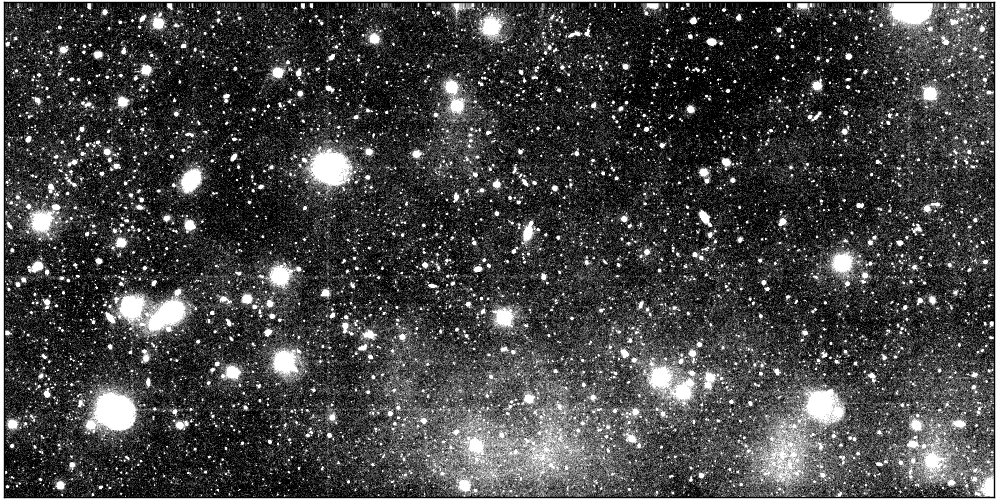
\includegraphics[width=0.7\textwidth]{detect-r-00} \\
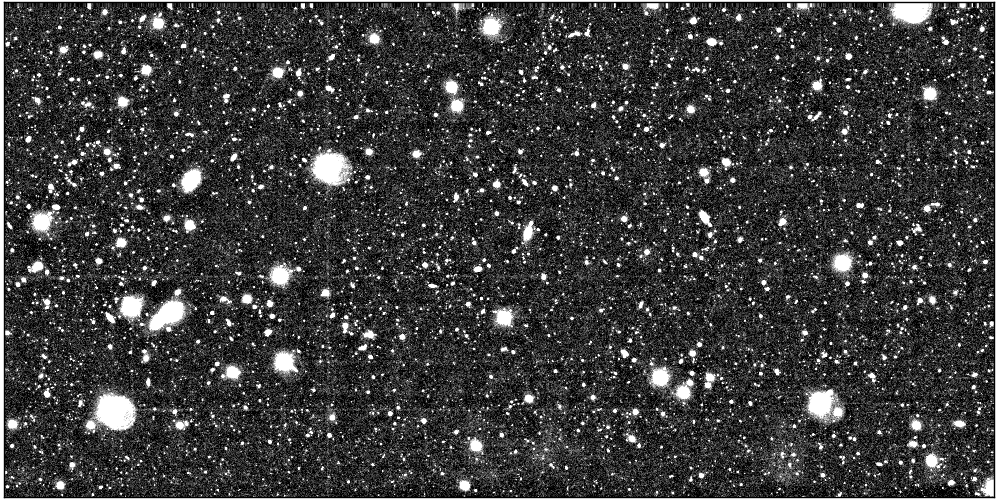
\includegraphics[width=0.7\textwidth]{detect-r-01} \\
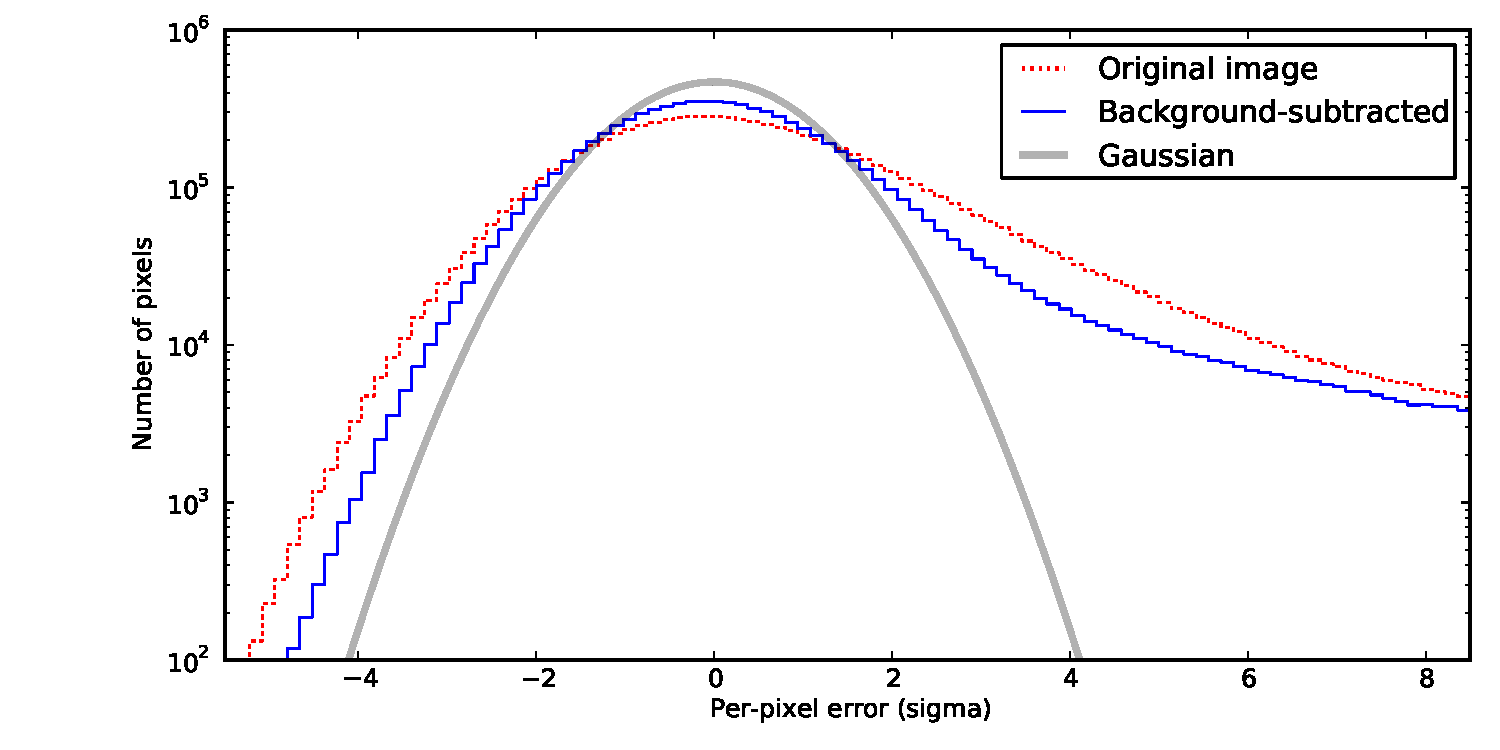
\includegraphics[width=0.8\textwidth]{detect-r-02}
\caption{Residual background subtraction.  \textbf{Top:} combined
  \detmap\ for the SDSS $r$ band, combining images from 23 runs.
  There are clear patterns in the background level.  \textbf{Middle:}
  after estimating and removing the residual background as described
  in the text, the background appears more flat.  \textbf{Bottom:}
  after removing the background, the pixel error statistics are closer
  to Gaussian, though the distribution is still significantly
  broader than expected.\label{fig:bg}}
\end{center}
\end{figure}


\begin{figure}
\begin{center}
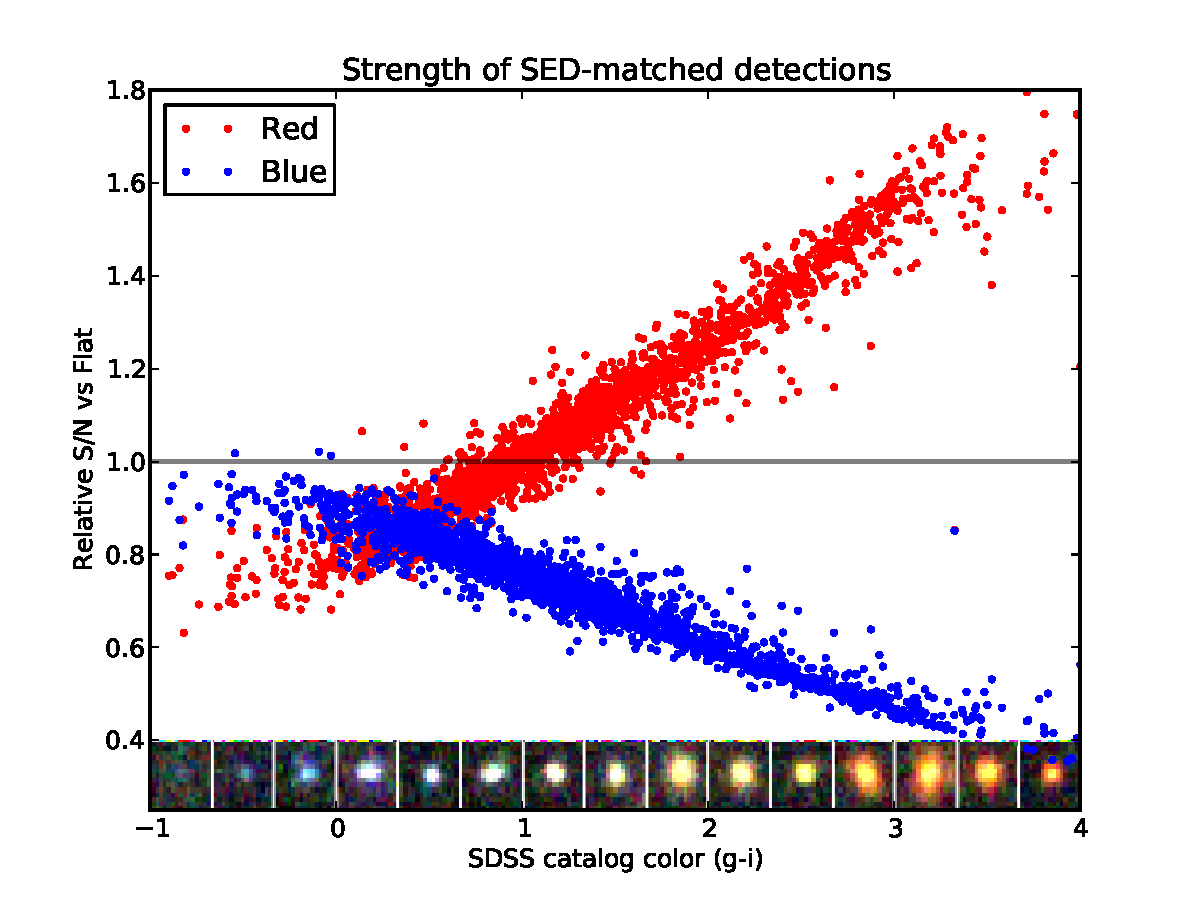
\includegraphics[width=0.8\textwidth]{mdetect-11}
\caption{Detection strengths in the Red, Flat, and Blue SED-matched
  filters, versus SDSS-measured colors.  We performed a spatial match
  between our detected sources and SDSS sources (from the DR7 CasJobs
  database ``Stripe82''; \cite{annis}) within 1 pixel.  Redder objects
  in $g-i$ are detected more strongly in the Red SED-matched filter
  than Flat or Blue.  The handful of objects with significantly blue
  colors are detected more strongly with the Blue filter.
  \label{fig:redblue}}
\end{center}
\end{figure}


\begin{figure}
\begin{center}
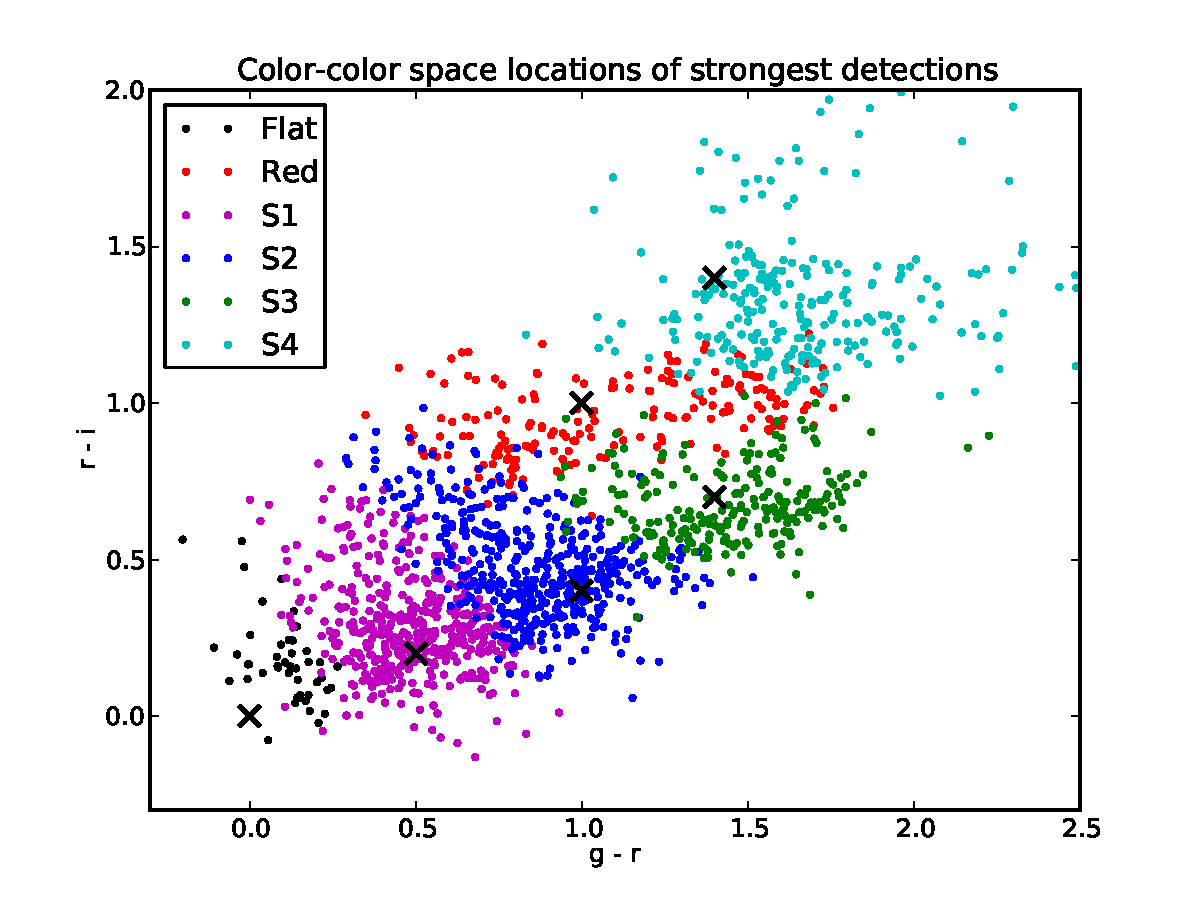
\includegraphics[width=0.8\textwidth]{mdetect-17}
\caption{Color-color space locations of sources detected most strongly
  by each of the filters.
  The color measurements are from the SDSS
  Stripe82 coadd catalog \cite{annis}, matched to
  our detections using a 1-pixel matching radius.
  It is clear that
  our different SED-matched filters are tuned to detect objects in
  particular regions of color-color space.  The ``X'' marks indicate
  the color each SED-matched filter is tuned for.  Note that many of
  the sources are detected above a given detection threshold by
  several of the SED-matched filters; here each source is assigned to
  the filter by which it is detected most strongly.
  \label{fig:colorcolor}}
\end{center}
\end{figure}


\begin{figure}
\begin{center}
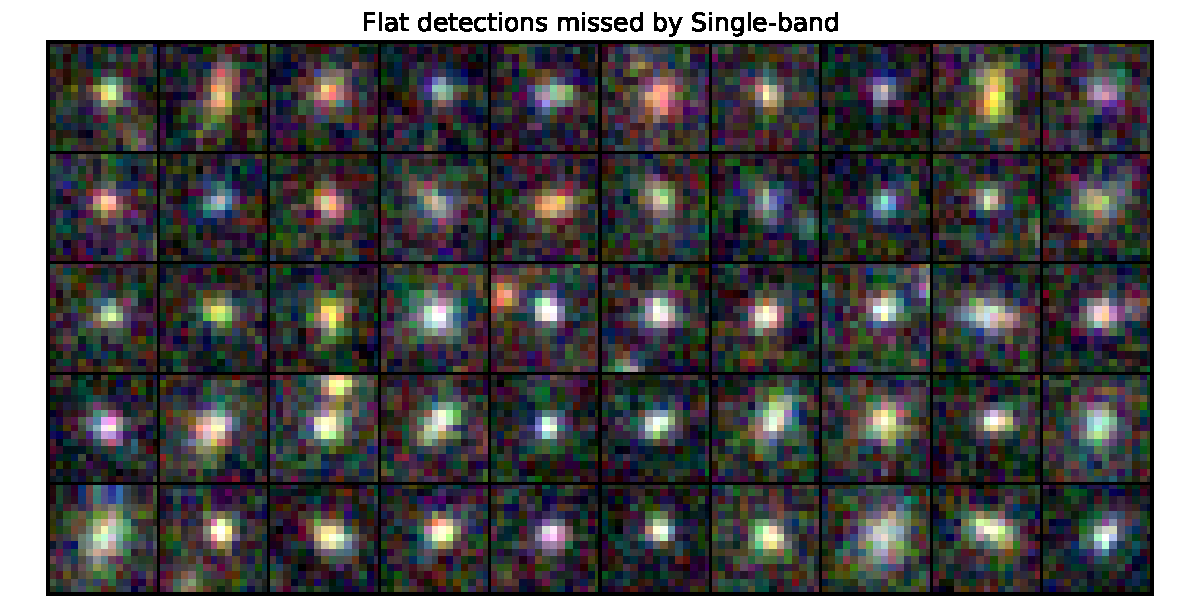
\includegraphics[width=0.8\textwidth]{mdetect-14}
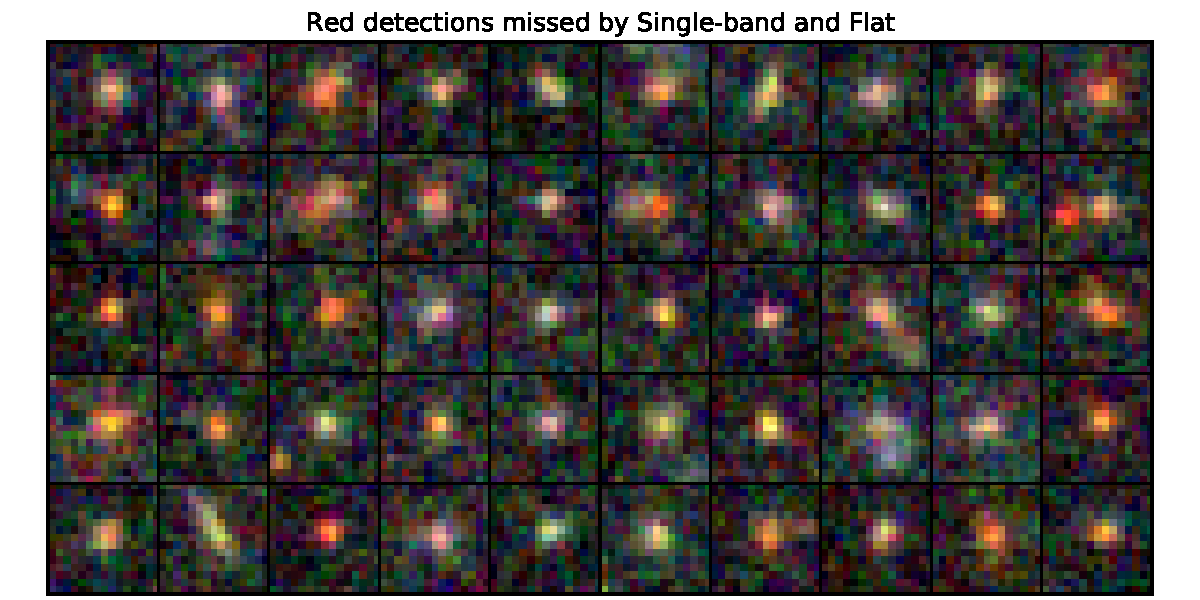
\includegraphics[width=0.8\textwidth]{mdetect-15}
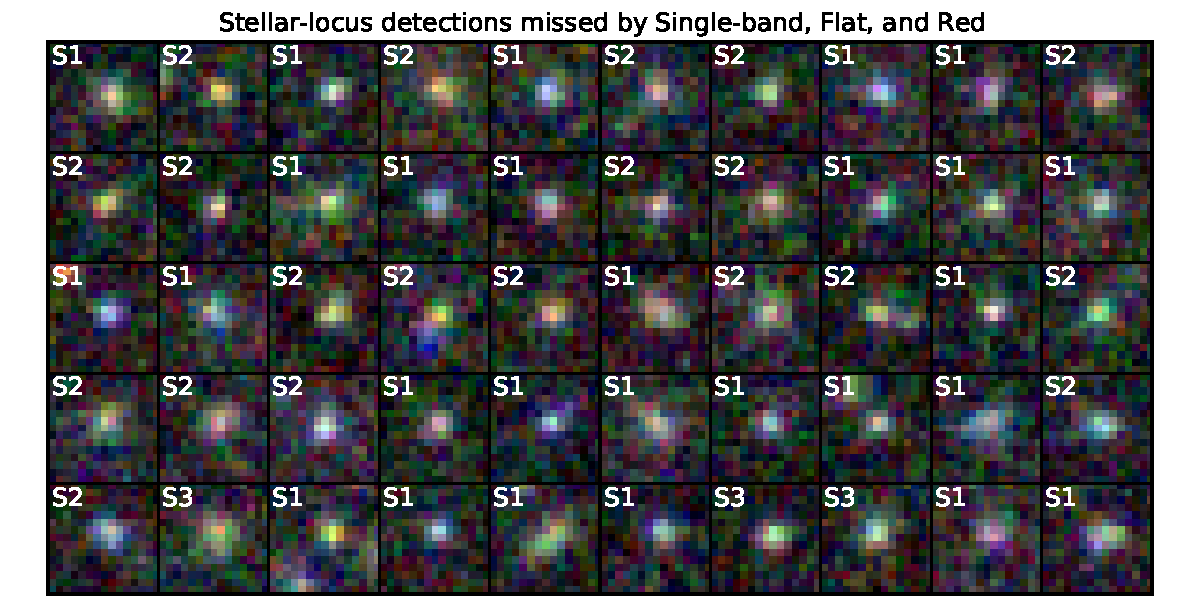
\includegraphics[width=0.8\textwidth]{mdetect-16}
\caption{Sources detected by our SED-matched filters and not by a
  ``traditional'' approach; full caption on next page\label{fig:missed}}
\end{center}
\end{figure}

\addtocounter{figure}{-1}
\begin{figure}
\begin{center}
\caption{[figure previous page] Sources detected by applying a
  sequence of SED-matched filters.  We start with sources detected by
  a ``traditional'' approach that takes the union of single-band
  detections in each of the $g$, $r$, and $i$ filters.  We then apply,
  in sequence, our Flat, Red, and Stellar locus SED-matched filters.
  Each panel shows the sources detected by the new filter and not
  detected by previous filters, in order of decreasing
  signal-to-noise.  In order to make the objects easier to see, we
  have increased the detection threshold to $20 \sigma$.}
\end{center}
\end{figure}

\begin{figure}
\begin{center}
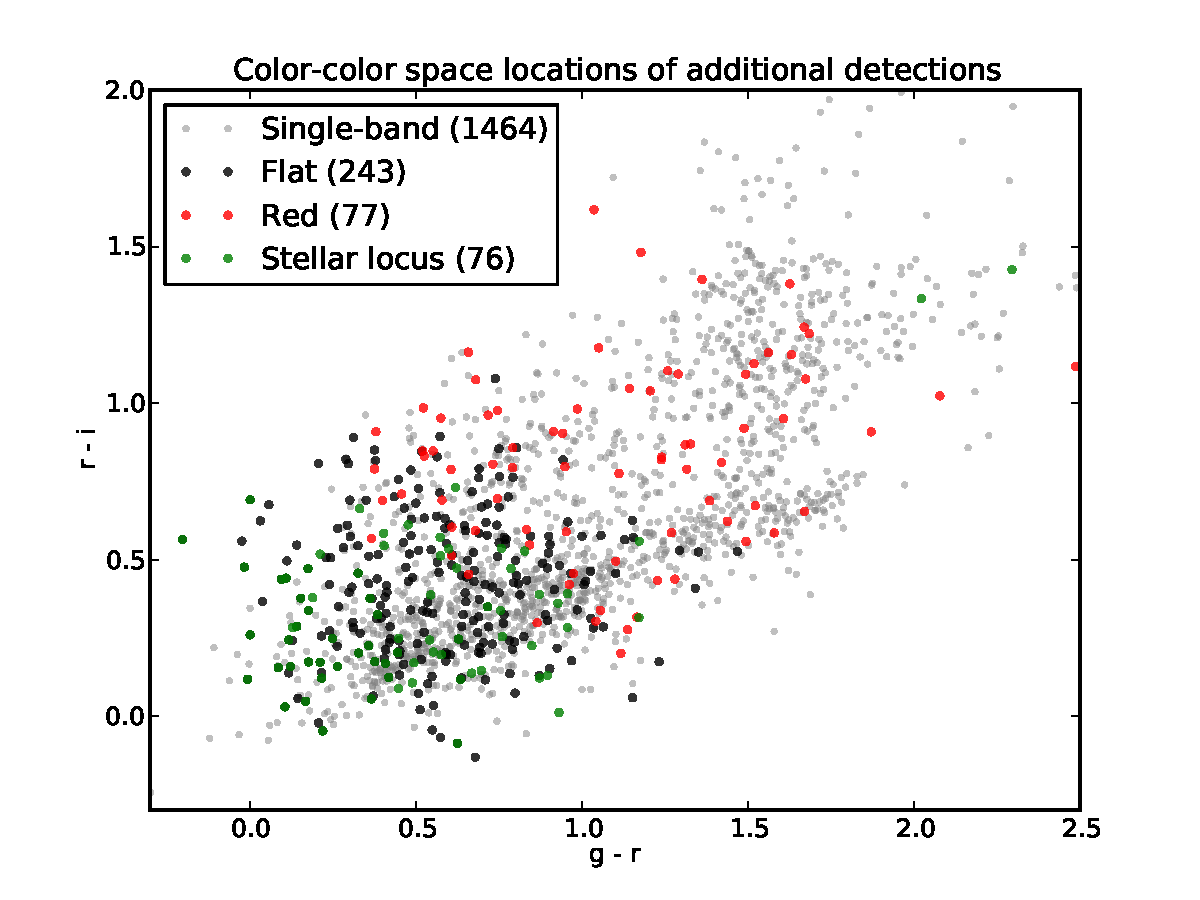
\includegraphics[width=0.8\textwidth]{mdetect-18}
\caption{Color-color space locations of additional sources detected as
  additional SED-matched filters are applied.  We start by taking all
  single-band detections in the $g$, $r$, and $i$-band filters.  Next,
  we add sources detected by the Flat SED-matched filter, then the Red
  filter, then a set of filters along the stellar locus.  Each
  subsequent SED-matched filter detects sources that are missed (at a
  fixed detection threshold) by the previous filters.
  %The color measurements are from the SDSS
  %Stripe82 coadd catalog \cite{annis}, matched to
  %our detections using a 1-pixel matching radius.
  \label{fig:added}}
\end{center}
\end{figure}




\section{Junk here}






different bandpass filters, with different sky noise levels, exposure
times, and point-spread functions.  How do we optimally detect the
source?  \commentout{ We first compute the \detmap\ for each image,
  then compute a weighted sum of the individual \detmap s to produce a
  \emph{total \detmap}.  }
%Since the noise in different images is independent, the maximum-like

\commentout{
In previous sections, we have seen that the signal-to-noise in a
\detmap\ $D_i$ at the true location of a source is proportional to:
\begin{equation}
\snr{D_i} \propto \frac{r_i \sqrt{t_i}}{w_i \sqrt{s_i}} \quad ,
\end{equation}
where $r_i$ is the count rate, given the filter and sensitivity of
image $i$, $t_i$ is the exposure time, $w_i$ is the ``width'' of the
point-spread function ($1/\norm{\psf}$, proportional to $w$ for a
Gaussian point-spread function with standard deviation $w$), and $s_i$
is the sky count rate (see equations \ref{eqn:sndsingle},
\ref{eqn:sndsinglegauss}, and \ref{eqn:snimg}).

As in previous sections, we combine these \detmap s, weighting
by their squared signal-to-noise, to find the total \detmap\ 
$D^\star$:
\begin{equation}
D^{\star} = \sum_i D_i \, \frac{r_i^2 \, t_i}{w_i^2 \, s_i}
\end{equation}
}



%To begin, we must produce a likelihood function.
%Since the noise in each image is independent, the likelihood g

We saw in previous sections that source detection is essentially the
same as estimating the flux of the putative source at a given source
position.  Given multi-band data, we must assume a spectral energy
distribution (or set of colors in the available filters) for the
source to be detected.  This is exactly parallel to the assumption
that we have a good model of the point-spread function; in both cases
we are constructing a matched filter.

Given an SED, we can either produce an estimate of the amplitude, or
equivalently estimate the source counts in a canonical filter.




%[[In practice, you can get away with approximate SED models (as with
%    approximate PSF models); suck it up, cut at $4 \sigma$ rather than
%    $5 \sigma$ and pick up the pieces later]]

%[[What's the S/N of that detection image; show that it's optimal (assuming it is!)]]


\newpage



\section{Co-adding images}

First, it should be noted that co-adding a stack of images is usually
not the Right Thing to do (cite Hogg).  The various procedures that
are typically applied to produce co-adds do more or less violence to
the data in the name of expediency.  Here we simply lay out the
conditions under which it is appropriate to co-add images (noting that
they rarely if ever occur in practice) and show how images should be
co-added in that case.


In the simplest case, we have a series of images taken through the
same bandpass filter with perfectly aligned pixels, identical PSF and
identical sky noise (which, as in the previous section, we will assume
is pixelwise independent, with zero mean and constant variance), and
no read noise.  Assume also that the sources in the image have no
proper motion or parallax and have constant flux.  All that varies
between the images is the exposure time.  In this case, it turns out
that simply adding the images together results in no information loss.
% the co-added image has the same sufficient statistics as the


It may seem obvious that simply adding the images together is the
right thing to do: CCDs are linear devices (in this \doctype), so adding
the images together is like taking a single exposure for the sum of
the individual exposure times.
%  But why doesn't it help to have more
%samples?  Let us work through the proof.


%\begin{tabular}{rcl}
%$<$total source photons collected$>$ & $\propto$ & exposure time \\
%photo-electrons (``flux'')
%$<$total sky photons collected$>$ & $\propto$ & exposure time \\
%total sky photons collected & $\drawnfrom$ & $\mathrm{Poisson}(s \cdot (\mathrm{exposure time}))$ \\
%  & $\simeq$ & $\gaussian{s t, s t}$ \\
%total sky noise & $\propto$ & $\sqrt{s t}$ \\
%\end{tabular}

For each pixel $\jvec$ in the image, the \emph{expected} (mean) number
of counts from the source, $\expect{C_{\jvec}}$, is equal to the count
rate $r_{\jvec}$ times the exposure time $t$.  Note that the source
counts are also the result of stochastic processes, so will by drawn
from some distribution of their own, but we will assume that the noise
in our images is dominated by the sky background, so we will consider
only the mean of the source distribution:
\begin{equation}
\expect{C_{\jvec}} = r_{\jvec} \, t \quad .
\end{equation}
Meanwhile, the sky contributes a mean count rate of $s$ counts per
unit time per pixel, yielding a total number of sky counts $S$ per
pixel,
\begin{eqnarray}
\expect{S} &=& s \, t \\
S & \drawnfrom & \mathrm{Poisson}(s \, t) \\
S & \simeq & \gaussian{s \, t, s \, t}
\end{eqnarray}
so the signal-to-noise is:
\begin{eqnarray}
\snr{\jvec} & = & \frac{\expect{C_{\jvec}}}{\sqrt{\var{S}}} \\
& = & \frac{r_{\jvec} \, t}{\sqrt{s \, t}} \\
& = & \frac{r_{\jvec} \sqrt{t}}{\sqrt{s}} \quad .
\label{eqn:snimg}
\end{eqnarray}
%note that we have assumed that the mean sky level $s \, t$ has been
%subtracted.
This is the well-known result that the signal-to-noise
increases as the square root of exposure time.


Consider two pixel-aligned images, $I_1$ and $I_2$, with different
exposure times, $t_1$ and $t_2$.  A linear combination of these
(sky-subtracted) images with the coefficients $\alpha_1$ and
$\alpha_2$ yields the image:
\begin{eqnarray}
  I &=& \alpha_1 I_1 + \alpha_2 I_2 \\
\label{eqn:imgsum}
& \drawnfrom & \alpha_1 \, \gaussian{r \, t_1, s \, t_1} + \alpha_2 \, \gaussian{r \, t_2, s \, t_2} \\
& \drawnfrom & \gaussian{r(\alpha_1 \, t_1 + \alpha_2 \, t_2) \,,\, s (\alpha_1^2 \, t_1 + \alpha_2^2 \, t_2)}
\end{eqnarray}
and the signal-to-noise in this image is:
\begin{equation}
\snr{I} = \frac{r (\alpha_1 \, t_1 + \alpha_2 \, t_2)}{\sqrt{s} \sqrt{\alpha_1^2 \, t_1 + \alpha_2^2 \, t_2}}
\end{equation}
which is optimized by setting $\alpha_1 = \alpha_2$ regardless of
$t_1$ and $t_2$; optimal signal-to-noise is achieved by simply adding
the image pixel values together.




\subsection{Comments}

\paragraph{Why equal weights?}
The result that images should just be added together with no uniform
weights should seem slightly surprising: if a longer exposure has
better signal-to-noise, shouldn't we weight it more heavily in the
co-add?  In effect, we \emph{have} done this: In the equations above,
we computed the \emph{total} source counts, not the counts per unit
time---we effectively weighted each image by its exposure time.
Recall that the exposure time is proportional to the square root of
signal-to-noise.  Thus, in effect we have co-added the images by
weighting each image by its squared signal-to-noise.

[ref appendix?]
\commentout{
To see this, again consider the case of combining two images, but
before doing so, let us convert the images to ``rate images'',
measured in units of counts per unit time:
\begin{equation} R_1 = I_1 / t_1 \qquad \mathrm{and} \qquad R_2 = I_2 / t_2 \quad . \end{equation}
We then get:
\begin{eqnarray}
  R &=& \alpha R_1 + (1 - \alpha) R_2 \\
  &=& \alpha \frac{I_1}{t_1} + (1 - \alpha) \frac{I_2}{t_2} \\
  &\drawnfrom& \frac{\alpha}{t_1} \gaussian{f t_1, \sky t_1} + \frac{1 - \alpha}{t_2} \gaussian{f t_2, \sky t_2} \\
  &\drawnfrom& \alpha \gaussian{f, \frac{\sky}{t_1}} + (1 - \alpha) \gaussian{f, \frac{\sky}{t_2}} \\
  &\drawnfrom& \gaussian{f, \frac{\alpha^2 \sky}{t_1} + \frac{(1 - \alpha)^2 \sky}{t_2}}
\end{eqnarray}
which has signal-to-noise
\begin{eqnarray}
\snr{R} &=& \frac{f}{\sqrt{\frac{\alpha^2 \sky}{t_1} + \frac{(1-\alpha)^2 \sky}{t_2}}} \\
\end{eqnarray}
which is optimized at
\begin{equation}
\alpha = \frac{t_1}{t_1 + t_2} \quad .
\label{eqn:snexptime}
\end{equation}
In other words, we must weight the rate images by their exposure
times, which is equivalent to their squared signal-to-noise.
}

\paragraph{Different sky.}
We assumed that the sky rate $s$ was equal in the images to be
co-added.  If this is not the case, then equation \ref{eqn:imgsum} can
be applied but with $s_1$ and $s_2$ replacing $s$.  The result is that
the images should be combined with the coefficients
\begin{equation}
\frac{\alpha_1}{\alpha_2} = \frac{s_2}{s_1} \qquad .
\end{equation}
This is not surprising, since we have seen that we must weight the
images by their signal-to-noise-squared, and from equation
\ref{eqn:snimg} we know that this goes as the inverse of the sky rate.

\paragraph{Different PSF.}
Above, we have assumed that the point-spread function is identical in
the two images.  How should the images be co-added if it is not?
First, we must ask what quantity we wish to optimize.  If we are
interested in detecting point sources, then we wish to optimize the
signal-to-noise in the co-added \detmap.  Assume that we have a good
PSF model for each of the two images $I_1$ and $I_2$.  We combine them
with coefficients $\alpha$:
\begin{equation}
  I_c = \alpha_1 I_1 + \alpha_2 I_2
\end{equation}
so the combined image $I_c$ has a point-spread function:
\begin{equation}
  \psf_c = \frac{\alpha_1 \psf_1 + \alpha_2 \psf_2}{\alpha_1 + \alpha_2} 
  \quad .
\end{equation}
The per-pixel sky noise variance in the combined image, $\sigma^2_c$, is
\begin{equation}
  \sigma^2_c = \alpha_1^2 \sigma_1^2 + \alpha_2^2 \sigma_2^2 \quad .
\end{equation}
We will assume equal sky variances: $\sigma = \sigma_1 = \sigma_2$.


From equation \ref{eqn:sndsingle}, the co-added \detmap\ has
signal-to-noise:
\begin{eqnarray}
\snr{D_c} &=& \frac{C (\alpha_1 + \alpha_2) \norm{\psf_c}}{\sigma_c} \\
&=& \frac{C (\alpha_1 + \alpha_2) \norm{\alpha_1 \, \psf_1 + \alpha_2 \, \psf_2}}{\sqrt{\sigma_1^2 (\alpha_1^2 + \alpha_2^2)}} \quad .
%&\propto& \frac{\sqrt{\sum_{x,y} \left( \alpha \, \psf_1 + (1-\alpha) \, \psf_2 \right)^2}}{\sqrt{\alpha^2 + (1-\alpha)^2}} \quad .
\end{eqnarray}

Assuming Gaussian point-spread functions with standard deviations
$w_1$ and $w_2$, we get
\begin{eqnarray}
%\left( \snr{D_c^G} \right)^2 &\propto& 
%\frac{\sum_{x,y} \left(
%  \alpha \, \frac{1}{2 \pi w_1^2}\exp{\left(-\frac{x^2+y^2}{2 w_1^2}\right)}
%  + (1-\alpha) \, \frac{1}{2 \pi w_2^2}\exp{\left(-\frac{x^2+y^2}{2 w_2^2}\right)}
%\right)^2}{\alpha^2 + (1-\alpha)^2}
%
\left[ \snr{D_c^G} \right]^2 &\propto&
\frac{(\alpha_1 + \alpha_2)^2 \left(
  \frac{\alpha_1^2 \norm{\psf_1}^2 + \alpha_2^2 \norm{\psf_2}^2 + 2 \alpha_1 \alpha_2 \sum_{\ivec} \psf_1(\ivec) \psf_2(\ivec)}%
       {(\alpha_1 + \alpha_2)^2}
\right)}
{\alpha_1^2 + \alpha_2^2} \\
%
&\simeq&
\frac{%
  \frac{\alpha_1^2}{4 \pi w_1^2}  +
  \frac{\alpha_2^2}{4 \pi w_2^2}  +
  2 \alpha_1 \alpha_2 \displaystyle\iint
  %\frac{1}{4 \pi^2 w_1^2 w_2^2}
  %\exp{\left(-\frac{x^2+y^2}{2 w_1^2}\right)}
  %\exp{\left(-\frac{x^2+y^2}{2 w_2^2}\right)}
  \gaussx{x^2 + y^2 \,,\, w_1^2} \gaussx{x^2 + y^2 \,,\, w_2^2}
  \mathrm{d}x \, \mathrm{d}y}%
     {\alpha_1^2 + \alpha_2^2} \\
&\propto&
\frac{%
  \displaystyle\frac{\alpha_1^2}{w_1^2}  +
  \displaystyle\frac{\alpha_2^2}{w_2^2}  +
  \displaystyle\frac{4 \alpha_1 \alpha_2}{w_1^2 + w_2^2}%
}{\alpha_1^2 + \alpha_2^2}
%
%  \alpha \, \frac{1}{2 \pi w_1^2}\exp{\left(-\frac{x^2+y^2}{2 w_1^2}\right)}
%  + (1-\alpha) \, \frac{1}{2 \pi w_2^2}\exp{\left(-\frac{x^2+y^2}{2 w_2^2}\right)}
%\right)^2}{\alpha^2 + (1-\alpha)^2}
\end{eqnarray}
which has extrema at
\begin{equation}
\frac{\alpha_2}{\alpha_1} = \frac{w_1^4 - w_2^4 \pm \sqrt{w_1^8 + 14 \, w_1^4 w_2^4 + w_2^8}}{4 \, w_1^2 w_2^2}
\end{equation}
(which we found with the help of Sage). %\cite{sage}).


By defining $\omega = w_2 / w_1$, we get the simpler expression:
\begin{equation}
  \frac{\alpha_2}{\alpha_1} = \frac{1 - \omega^4 \pm \sqrt{\omega^8 + 14 \, \omega^4 + 1}}{4 \, \omega^2}
  \label{eq:coaddwt1}
\end{equation}
which is still strikingly complex, but shows the expected behavior as
illustrated in \figref{fig:coaddwt1}.


\section{Discussion}

--talk about uncertainties in PSF, noise model, flat field / calibration,
source SEDs.  Extended sources.  Time varying?

--similarities and differences from Szalay et al 19999 -- SED-matched
filters $\sim$ ``optimal subspace filtering''

--galaxy detection?

--No weights go to zero -- all images contribute *something*, in
proportion to t he information they bring.  Contrast with lucky
imaging and some co-adding schemes.

--sub-pixel shifts: lower threshold so that max pixel is above
threshold; post-process to cut out peaks that really were below
threshold.


\section{Conclusions}

[[What to do with a detection image; how to proceed.  Build models,
    fit simultaneously to all images in the ``stack''.]]

[[Practicalities: bad pixels / masks, interpolation, etc]]


%\bibliographystyle{plain}
%\bibliography{coadd}

\begin{thebibliography}{70}
\raggedright

\bibitem[Ahn \etal(2012)]{dr9}
Ahn,~C.~P. \etal, \apjs, 203, 21

\bibitem[Annis \etal(2014)]{annis}
Annis, J. \etal, \apj, 792, 120

\bibitem[Blanton \etal(2007)]{kcorrect}
Blanton,~M.~R. \and Roweis,~S, \aj, 133, 734

\bibitem[Lupton \etal(2001)]{photo}
Lupton,~R.~H. \etal, ADASS X, 269 %; \arxiv{astro-ph/0101420}

\bibitem[Postman \etal(1996)]{postman}
Postman, M. \etal, 1996, \aj, 111, 615

%\bibitem[Stein \etal(2010)]{sage}
%Stein, W.~A. \etal, \emph{Sage

\bibitem[Stoughton \etal(2002)]{sdss-edr}
Stoughton, C. \etal, 2002, \aj, 123, 485

\bibitem[Szalay \etal(1999)]{szalay}
Szalay, A. \etal, 1999, \aj, 117, 68

\bibitem[Willman \etal(2002)]{willman}
Willman, B. \etal, 2002, \aj, 123, 848

\bibitem[York \etal(2000)]{sdss}
York,~D.~G. \etal, 2000, \aj, 120, 1579

\end{thebibliography}


\appendix

\section{Appendices}

\subsection{Image model}
\label{app:model}
%%% FIXME:
%%%---I think we assume 100% fill factor also
%%%---and well-sampled images?

%%% HOGG SAY: we assume *either* well sampled *or* complete fill factor.

% To begin, let us assume we have an image containing a point source
% that we wish to detect.  Assume that the image contains additive
% Gaussian noise that is independent (uncorrelated) between pixels and
% equal in variance.  This is roughly equivalent to assuming that the
% noise in the image is dominated by sky noise or read noise, rather
% than Poisson noise from the source itself.  This is close to correct
% at the limit of detecting faint sources in wide-band optical images.
% Also assume that we have a good model of the point-spread function,
% and that it is constant over the image.  Further, let us assume that
% the image has had the sky and other ``background'' levels removed so
% that the mean value would be zero if the image did not contain any
% sources.  

We consider astronomical images such as those obtained from an
(idealized) CCD.  Aside from noise, each pixel contains a signal
related to the number of photons incident upon it during the exposure.
%
We are measuring the intensity field $I(\thetavec,\posvec,\lambda,t)$
(energy per unit solid angle, two-dimensional transverse position,
wavelength, and time) by taking an exposure for some amount of time
through a filter, optics, and possibly atmosphere.  This can be seen
as an integration over time, wavelength, telescope aperture, and the
point-spread function.
%
% We model the signal $C_{\jvec}$ as being related to the intensity
% field $I(\thetavec,\posvec,\lambda,t)$ (energy per unit solid angle,
% two-dimensional transverse position, wavelength, and time) by a
% six-dimensional integral
Consider a discrete image made up of a square array of pixels $\jvec$,
each of which has signal (or counts) $C_{\jvec}$, where we use $\jvec$
as a two-dimensional focal-plane position, measured in pixel units.
The signal $C_{\jvec}$ is given by the integral
\begin{eqnarray}\displaystyle
%C_{\jvec} &=& \frac{\dd C}{\dd E}\,\int\dd^2\thetavec'\,\psi(\thetavec_{\jvec} - \thetavec')\,\int \dd^2\posvec\,A(\posvec)\int \dd\lambda\,\lambda\,R(\lambda)\,\int\dd t\,H(t)\,I(\thetavec',\posvec,\lambda,t) + \noise_{\jvec}
%\\
%C_{\jvec} &=& \frac{\dd C}{\dd E}\,\int \dd^2\cvec\,\psi(\jvec - \cvec)\,\Omega_1\,\int \dd^2\posvec\,A(\posvec)\,\int \dd\lambda\,\lambda\,R(\lambda)\,\int\dd t\,H(t)\,I(\thetavec_{\cvec},\posvec,\lambda,t) + \noise_{\jvec}
C_{\jvec} &=& \frac{\dd C}{\dd E}\,\Omega_1\, %
\!
\int \!\!\!
\int \!\!\!
\int \!\!\!
\int
I(\thetavec_{\cvec},\posvec,\lambda,t)
\;H(t)\,
\dd t\,
\;
\lambda\,R(\lambda)\,
\dd\lambda\,
\;
A(\posvec)\,
\dd^2\posvec\,
\;
\psi(\jvec - \cvec)\,
\dd^2\cvec\,
 + \noise_{\jvec}
\quad,
\label{eqn:bigint}
\end{eqnarray}
where 
%
$\dd C/\dd E$ is the calibration factor taking integrated energies to per-pixel counts (in the mean),
%
$\Omega_1$ is the solid angle of a single pixel (assumed the same for all pixels),
%
$I(\cdot)$ is the intensity field,
%
$\thetavec$ is a two-dimensional angular position on the sky,
%
$t$ is a time, $H(t)$ is a function describing the time period over which the telescope was
integrating this exposure,
%
$\lambda$ is a wavelength, $R(\lambda)$ is a function describing the bandpass \citep{kcorrect},
%
$\posvec$ is a two-dimensional position vector in the telescope aperture plane,
%
$A(\posvec)$ is a function describing the telescope aperture,
%
$\psi(\cdot)$ is a function describing the pixel-convolved point-spread function of the
whole system,
%
$\cvec$ is a two-dimensional focal-plane position in the same coordinates and units as $\jvec$,
%
and
$\noise_{\jvec}$ is the noise contribution to pixel $\jvec$.
%
The per-pixel noise could include effects such as read noise and dark current.
%
Importantly, the PSF function is the pixel-convolved PSF, not simply
the PSF due to optics and atmosphere, so image pixels are a sampling
and not a convolution of the PSF-convolved intensity field.
%We will assume the PSF is well-sampled by the pixels.

In %what follows
the rest of this \doctype, we will assume that the (perhaps tiny) image of
interest contains only a uniform background value plus one point
source $k$ with some (unknown) flux $F_k$ and position $\thetavec_k$.
In this case, the intensity field is just
\begin{eqnarray}\displaystyle
I(\thetavec',\posvec,\lambda,t) &=& I_{\sky}(\lambda, t) + F_k(\lambda, t)\,\delta(\thetavec_k - \thetavec')
\quad,
\label{eqn:intensity}
\end{eqnarray}
where $I_{\sky}$ is the intensity of the background (sky), $F_k$ has
units of flux (energy per area per time per wavelength), and
$\delta()$ is a two-dimensional delta function on the sky.  For
simplicity, we have dropped all assumption-violating contributions
from galaxies, nebulosity, neighboring sources, or sky gradients.  The
noise values are drawn from a probability distribution which we assume
to be
\begin{eqnarray}\displaystyle
p(\noise_{\jvec}) &=& \gaussian{\noise_{\jvec}|0,\sigma_1^2}
\quad,
\end{eqnarray}
where $\gaussian{x|m,V}$ is the Gaussian distribution with mean $m$
and variance $V$, and $\sigma_1^2$ is the per-pixel noise variance
(assumed equal for all pixels).  That is, we are assuming constant,
zero-mean, Gaussian noise.  This assumption is not too bad for
sky-limited images from which the sky level has been subtracted: the
sky contribution can be modeled as a Poisson process contributing
Poisson or ``shot'' noise which we then approximate by the Gaussian.
This approximation gets better as the sky level (number of
photo-electrons) increases.

In the above, we have made extremely strong assumptions.  In addition
to the listed assumptions we have assumed that any electronic gain at
readout has been calibrated out.  We have also assumed that the image
is not contaminated by cosmic rays, stray light, bad pixels, bad
columns, electronic artifacts, or any other of the many defects in
real images.



\subsection{Optimal linear detection}
\label{app:lindet}

Let us assume that there exists a linear filter whose output allows
optimal detection of isolated point sources.  That is, we seek a
(two-dimensional) set of coefficients $a_{\ivec}$ that, when
correlated with the image $S_{\jvec}$, produces a map $M_{\jvec}$
whose peak is the likely location of the point source.  See
\figref{fig:detmap}.


The linear filtering (correlation) operation is
\begin{equation}
M_{\jvec} = \sum_{\iina} a_{\ivec} \, S_{\ivec + \jvec}
\label{eq:detmap1}
\end{equation}
where $\mathcal{A}$ is the support of $\avec$ (integer pixel
positions), and the center of $\avec$ is $\coord{0}{0}$.  We will
demand that the elements of $\avec$ are non-negative and sum to unity.

Inserting \eqnref{eq:modelimg}, we get
\begin{eqnarray}
M_{\jvec} &\drawnfrom& \sum_{\iina}
  C_k \, a_{\ivec} \, \psi(\ivec + \jvec - \kvec) + \gaussx{0, \sigma_1^2}
  \\
&\drawnfrom& \gaussx{ C_k \sum_{\iina} a_{\ivec} \, \psi(\ivec + \jvec - \kvec),
    \sum_{\iina} a_{\ivec}^2 \, \sigma_1^2}
\end{eqnarray}
and the per-pixel signal-to-noise in the map is
\begin{equation}
%  \signoise_{D_{\jvec}} = \frac{C_k \, \sum_{\iina} a_{\ivec} \, \psi(\ivec + \jvec - \kvec)}{\sigma_1 \sqrt{\sum_{\iina} a_{\ivec}^2}}
  \snr{M_{\jvec}} = \frac{C_k \, \sum a_{\ivec} \, \psi(\ivec + \jvec - \kvec)}{\sigma_1 \sqrt{\sum_{\ivec} a_{\ivec}^2}} \quad .
  \label{eq:detmapsn1}
\end{equation}

We want to choose coefficients $a_{\ivec}$ to maximize the 
signal-to-noise at the true pixel position of the source,
$\kvec$.  Rewriting the expression using dot-products and
norms\footnote{All norms in this \doctype\ are $\ell_2$ norms: $\norm{X} =
  \sqrt{\sum_i X_i^2}$.}, treating the two-dimensional images
$a_{\ivec}$ and $\psi(\ivec + \jvec - \kvec)$ as vectors indexed by
$\ivec$, we have:
\begin{eqnarray}
  %\signoise_{D_{\jvec}} &=& \frac{C_k \, \avec \cdot \bm{\psi(\jvec-\kvec)}}{\sigma_1 \sqrt{\avec \cdot \avec}} \\
  \snr{M_{\jvec}} &=& \frac{C_k \, \avec \cdot \bm{\psi(j-k)}}{\sigma_1 \sqrt{\avec \cdot \avec}} \\
 &=& \frac{C_k \, \norm{\avec} \norm{\bm{\psi(j-k)}} \cos \theta}{\sigma_1 \norm{\avec}} \\
 &=& \frac{C_k \, \norm{\bm{\psi(j-k)}} \cos \theta}{\sigma_1}
\end{eqnarray}
where $\theta$ is a generalized angle between $\avec$ and $\bm{\psi(j-k)}$.
At the pixel position of the source, $\kvec$,
\begin{equation}
\snr{M_{\kvec}} = \frac{C_k \, \norm{\bm{\psi(0)}} \cos \theta}{\sigma_1}
\label{eqn:sndsingle}
\end{equation}
Clearly this is maximized when $\theta = 0$, \ie, when $\avec$ is a
multiple of $\bm{\psi(0)}$, the PSF evaluated at a grid of integer
pixel positions.  Since we have defined both the PSF and coefficients
$a$ to sum to unity, we find that the optimal linear filter for
detection is given by:
\begin{equation}
%  a_{\ivec} = \psi_{\ivec} \quad ,
\avec = \bm{\psi(0)} \quad ,
\end{equation}
which means that the operation of \emph{correlating} the image with
its PSF produces a map with optimal signal-to-noise.  Repeating
equation \ref{eq:detmap1}, we have found that the map $M_{\jvec}$ can
be computed by correlating the image with its PSF:
\begin{equation}
M_{\jvec} = \sum_{\iina} \psi_{\ivec} \, S_{\ivec + \jvec} \quad ,
\end{equation}
where, as before, $\mathcal{A}$ is the support of the PSF and
$\psfat{\ivec} = \psi(\ivec)$ is an image of the PSF evaluated at
integer pixel positions $\ivec$.

The signal-to-noise in this map at the true source pixel
position $\kvec$ is
\begin{equation}
\snr{M_{\kvec}} = \frac{C_k \, \norm{\bm{\psi}}}{\sigma_1} \quad .
\end{equation}



\subsubsection{Norm of a Gaussian PSF}
\label{app:gaussnorm}
For a Gaussian PSF with standard deviation $\psfw$ pixels,
\begin{eqnarray}\displaystyle
\psf^G(x,y) &=& \frac{1}{2 \pi \psfw^2} \exp{\left(-\frac{x^2}{2 \psfw^2}\right)} \exp{\left(-\frac{y^2}{2 \psfw^2}\right)}
\end{eqnarray}
the norm is% approximately:
\begin{eqnarray}
\norm{\bm{\psf^G}} &=& \sqrt{ \sum_{x} \sum_{y} \left(\frac{1}{2 \pi \psfw^2} \exp{\left(-\frac{x^2}{2 \psfw^2}\right)} \exp{\left(-\frac{y^2}{2 \psfw^2}\right)} \right)^2} \\
%\left(\norm{\psf^G}\right)^2 &\simeq& \iint \frac{1}{4 \pi^2 \psfw^4} \exp{\left(-\frac{x^2}{\psfw^2}\right)} \exp{\left(-\frac{y^2}{\psfw^2}\right)} \mathrm{d}x \, \mathrm{d}y \\
\norm{\bm{\psf^G}} &\simeq& \sqrt{\iint \frac{1}{4 \pi^2 \psfw^4} \exp{\left(-\frac{x^2}{\psfw^2}\right)} \exp{\left(-\frac{y^2}{\psfw^2}\right)} \mathrm{d}x \, \mathrm{d}y} \\
\norm{\bm{\psf^G}} &\simeq& \frac{1}{2 \sqrt{\pi} \psfw}
\end{eqnarray}
so the \detmap\ has signal-to-noise at the true source position $\kvec$,
\begin{equation}
\snr{D_{\kvec}^G} = \frac{C_k}{2 \sqrt{\pi} \psfw \sigma_1 } \quad .
\label{eqn:sndsinglegauss}
\end{equation}

Note, however, that we have defined the point-spread function
$\psi(\cdot)$ to be the \emph{pixel-convolved} response, so it cannot
be exactly Gaussian if the pixel response is assumed to be a boxcar
function.  In practice, however, a two-dimensional Gaussian with
variance $v^2$ correlated with a two-dimensional boxcar function is
well approximated by a Gaussian with variance $v^2 + \frac{1}{12}$, as
long as $v \gtrsim \frac{1}{2}$.

% figure showing this?




\subsubsection{Why not signal-to-noise-squared?}
In correlating the image with the PSF, it looks like the
\detmap\ weights pixels by their signal-to-noise, rather than
signal-to-noise \emph{squared}.  This apparent conflict can be
resolved by scaling the pixel values so that each pixel is an estimate
of the same quantity.  That is, we want to estimate the total source
counts $C$, but the pixels contain estimates of the source counts
scaled by the PSF, $C \psf$; we must undo this scaling by multiplying
the pixels by $1/\psf$.

Given a source at position $\kvec$, we define the image $K$ whose
pixels each contain an estimate of the total source counts:
\begin{eqnarray}
  K_{\jvec} &=& \frac{1}{\psfat{\jvec-\kvec}} S_{\jvec}  \\
  K_{\jvec} &\drawnfrom& \frac{1}{\psfat{\jvec-\kvec}} \, \gaussian{C_k \, \psfat{\jvec-\kvec}\, , \, \sigma_1^2} \\
  K_{\jvec} &\drawnfrom& \gaussian{C_k \, , \, \frac{\sigma_1^2}{\psfat{\jvec-\kvec}^2}} \quad .
\end{eqnarray}

The signal-to-noise remains the same, since we have just scaled the
values:
\begin{eqnarray}
\snr{K_{\jvec}} &=& \frac{C_k \, \psfat{\jvec-\kvec}}{\sigma_1} \\
\snr{K_{\jvec}} &=& \snr{S_{\jvec}} \quad .
\end{eqnarray}


As before, the \detmap\ pixels are a linear combination of the
(shifted) pixels of the $K$ image with weights $b_{\ivec}$:
\begin{eqnarray}
D_{\jvec}^\star &=& \sum_{\ivec} b_{\ivec} \, K_{\ivec+\jvec} \\
&\drawnfrom& \sum_{\ivec} b_{\ivec} \, \gaussian{C_k \,,\, \frac{\sigma_1^2}{\psfat{\ivec+\jvec-\kvec}^2}} \\
&\drawnfrom& \gaussian{C_k \sum_{\ivec} b_{\ivec} \,,\, \sum_{\ivec} \frac{b_{\ivec}^2 \sigma_1^2}{\psfat{\ivec+\jvec-\kvec}^2}}
\end{eqnarray}
and the signal-to-noise in that \detmap\ at pixel $\kvec$ is
\begin{eqnarray}
\snr{D_{\kvec}^\star} &=& \frac{C_k \sum_{\ivec} b_{\ivec}}{\sigma_1 \sqrt{\sum_{\ivec} \frac{b_{\ivec}^2}{\psfat{\ivec}^2}}}
\end{eqnarray}
which is maximized by setting the $b_{\ivec}$
\begin{equation}
b_{\ivec} \propto \psfat{\ivec}^2 \quad :
\end{equation}
proportional to the signal-to-noise \emph{squared}, as expected.

% Derivative is
% d\snr{D_k^\star}/db_k = 
%  \[ \frac{f}{\sigma} [ \frac{1}{\sqrt{\sum_j \frac{b_j^2}{\psfat{j}^2}}}
%                       - \frac{(\sum_j b_j) b_k}{\psfat{j}^2 (\sum_j \frac{b_j^2}{\psfat{j}^2})^{3/2}} ]
% \]
%
% And through some seemingly circular math you get to:
% b_k = \psfat{k}^2 * ( \sum_j (b_j^2 / \psfat(j)^2) ) / (sum_j (b_j))
%
% (you can remove the b_k term from the sums over j if you want, with no effect.)
%
% So b_k = \alpha \psfat{k}^2; substituting that you get:
%
% b_k = \psfat{k}^2 * ( \sum_j ( (\psfat{j}^2 \alpha)^2 / \psfat{j}^2 ) / (sum_j (\psfat{j}^2 \alpha))
%     = \psfat{k}^2 * ( \alpha^2 \sum_j \psfat{j}^2 ) / (\alpha \sum_j(\psfat{j}^2))
%     = \psfat{k}^2 * \alpha












\begin{figure}[htb]
\begin{center}
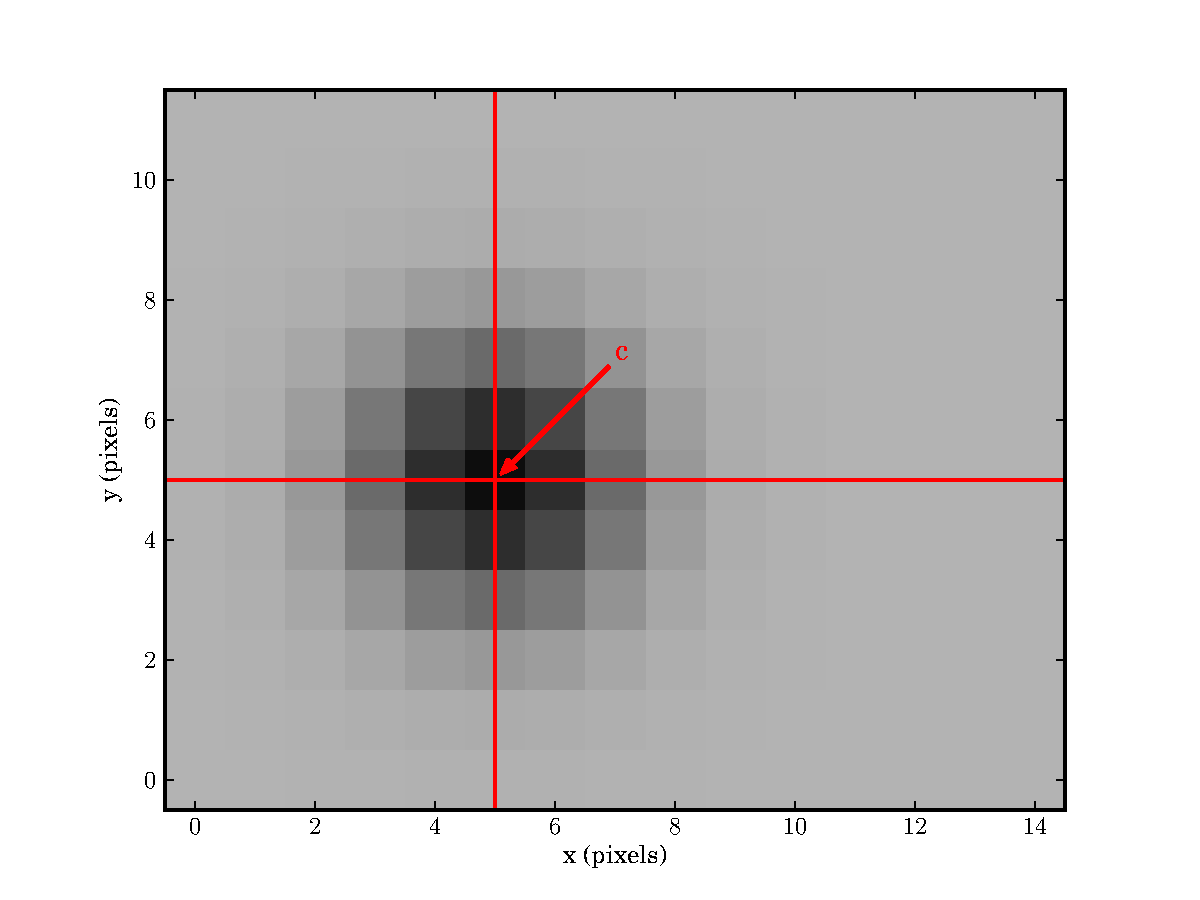
\includegraphics[width=0.3\textwidth]{f02d-bw}
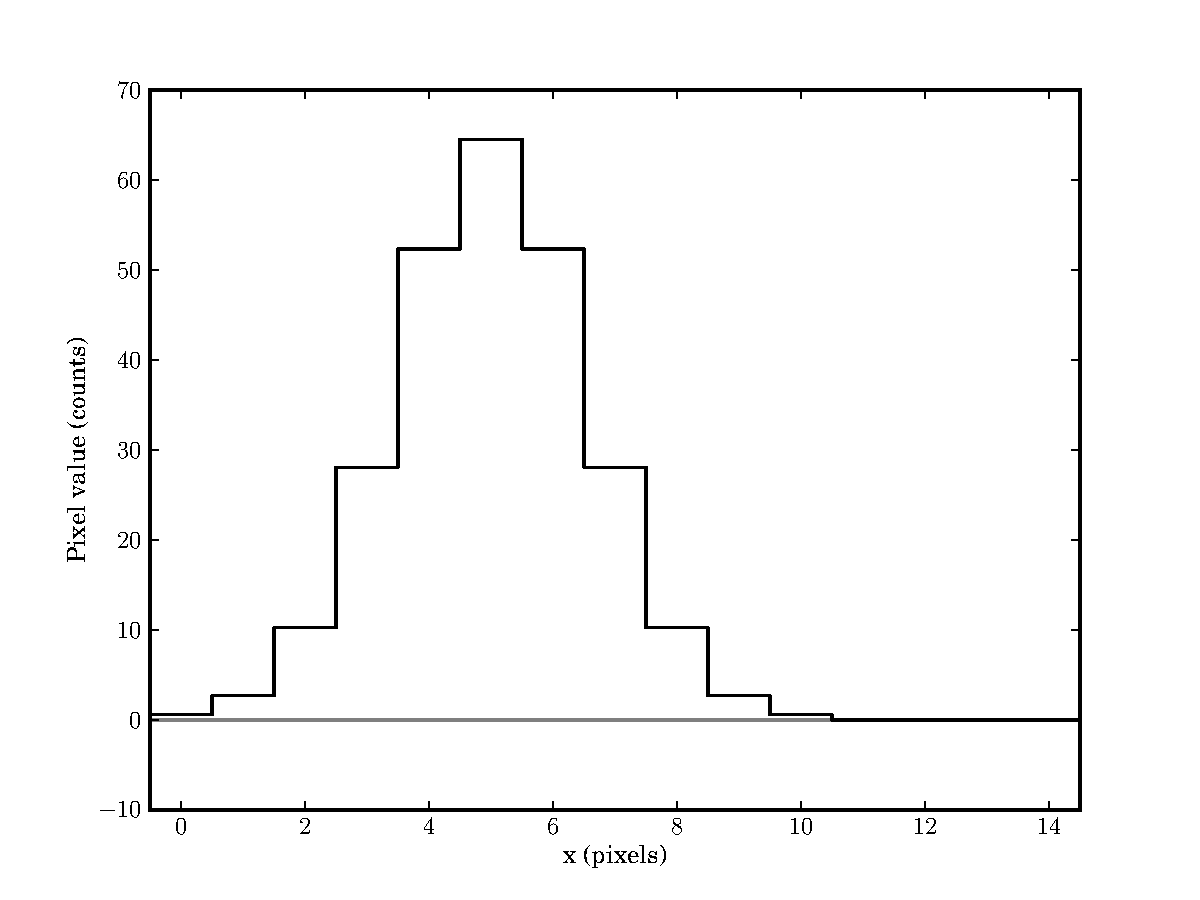
\includegraphics[width=0.3\textwidth]{f02g-bw} \\
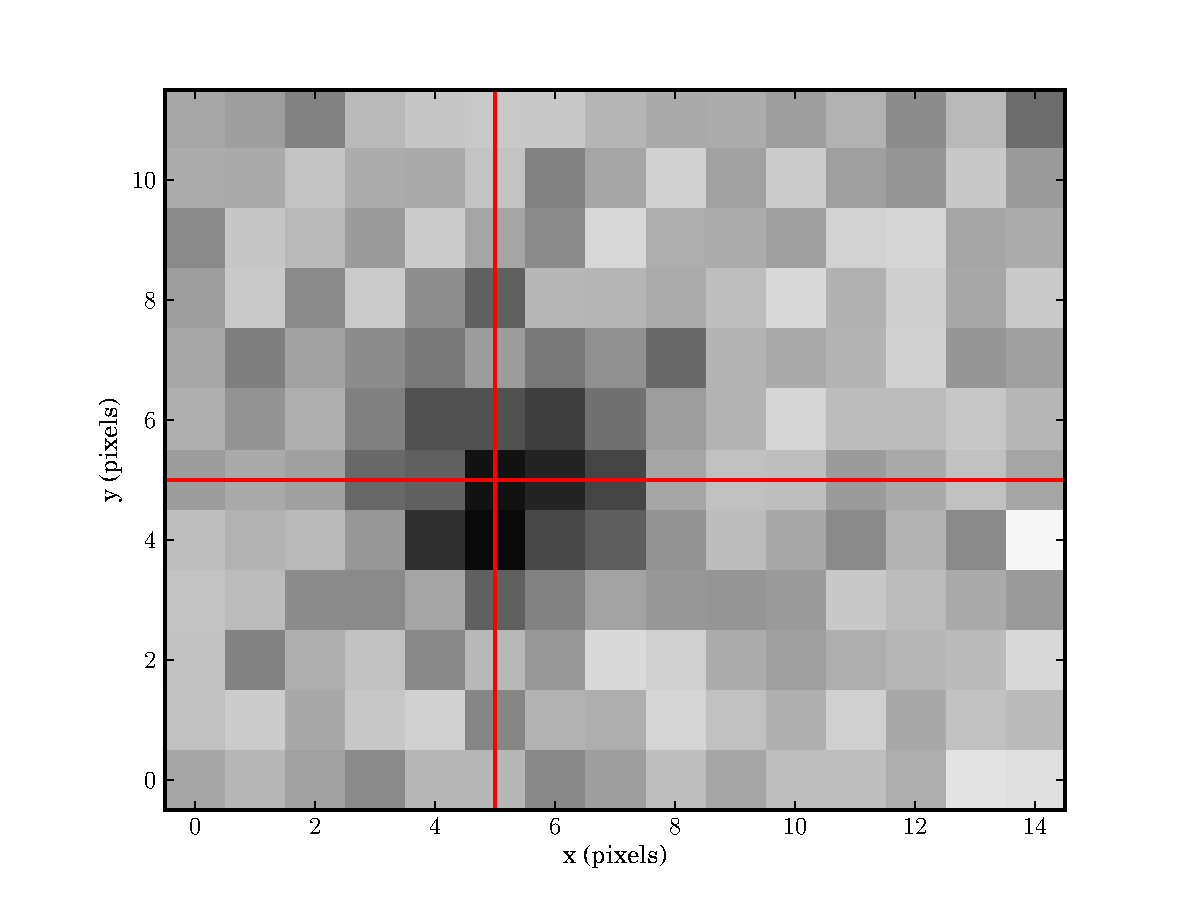
\includegraphics[width=0.3\textwidth]{f02e-bw}
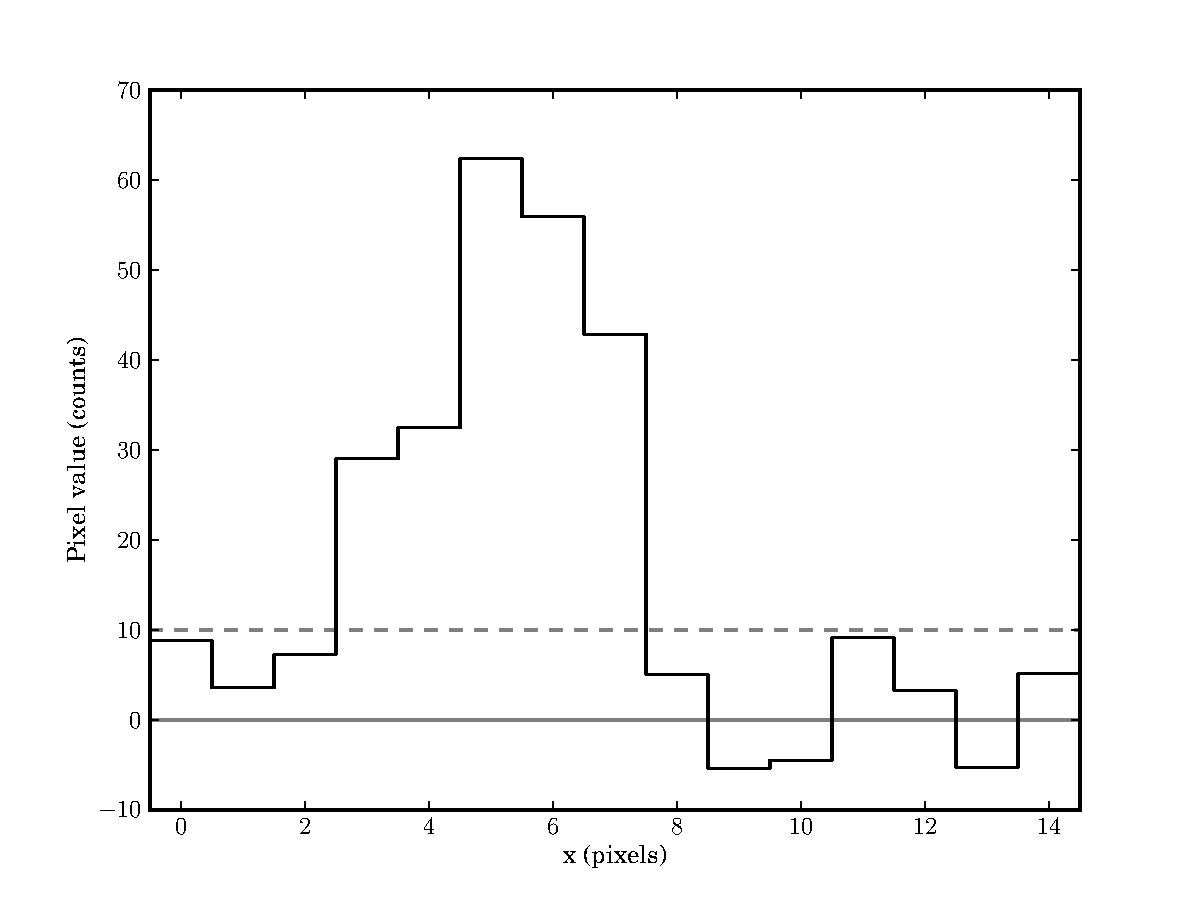
\includegraphics[width=0.3\textwidth]{f02h-bw}
\end{center}
\caption{An example image.  \figpart{Top-left:} without noise, with a
  source at an integer pixel offset, $\kvec = \coord{5}{5}$.  The
  image is simply a shifted version of the PSF function $\psi(\cdot)$
  sampled at pixel positions..  \figpart{Top-right:} slice through $y
  = 5$, the source centroid.  \figpart{Bottom-left:} with noise added.
  \figpart{Bottom-right:} slice through $y = 5$, with noise.  The
  dashed line shows the standard deviation $\sigma$ of the per-pixel
  noise.
\label{fig:image}}
\end{figure}


\begin{figure}[p!]
\begin{center}
  % ideal
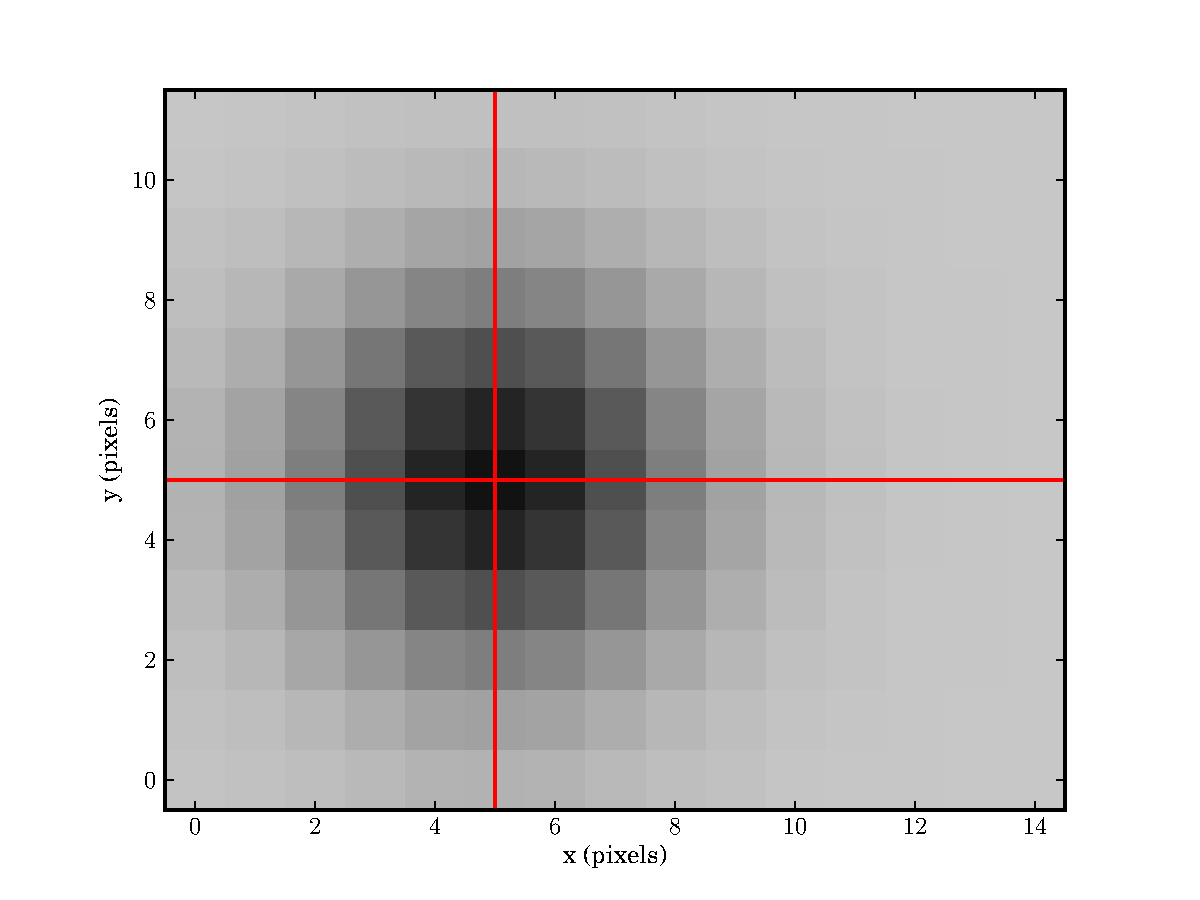
\includegraphics[width=0.3\textwidth]{f03c-bw}
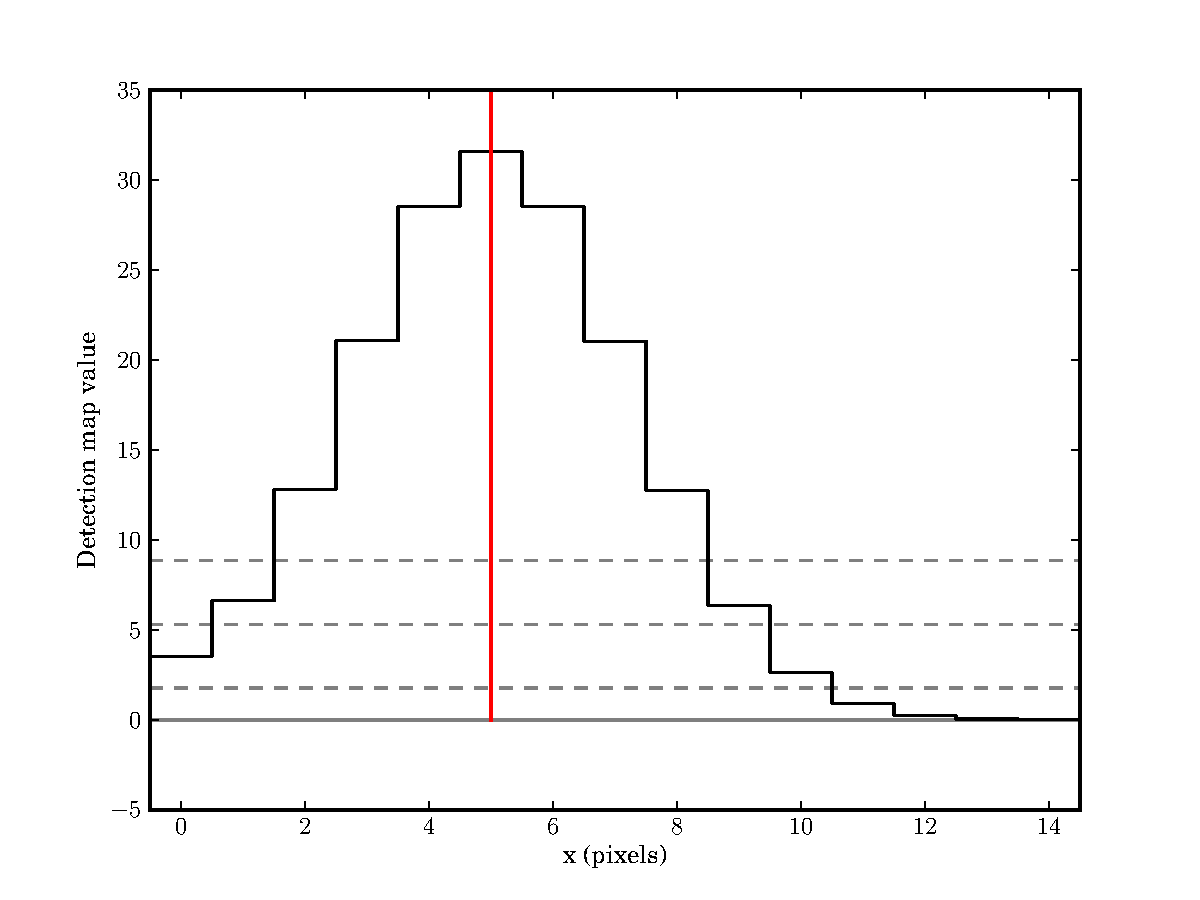
\includegraphics[width=0.3\textwidth]{f03d-bw} \\
% noisy
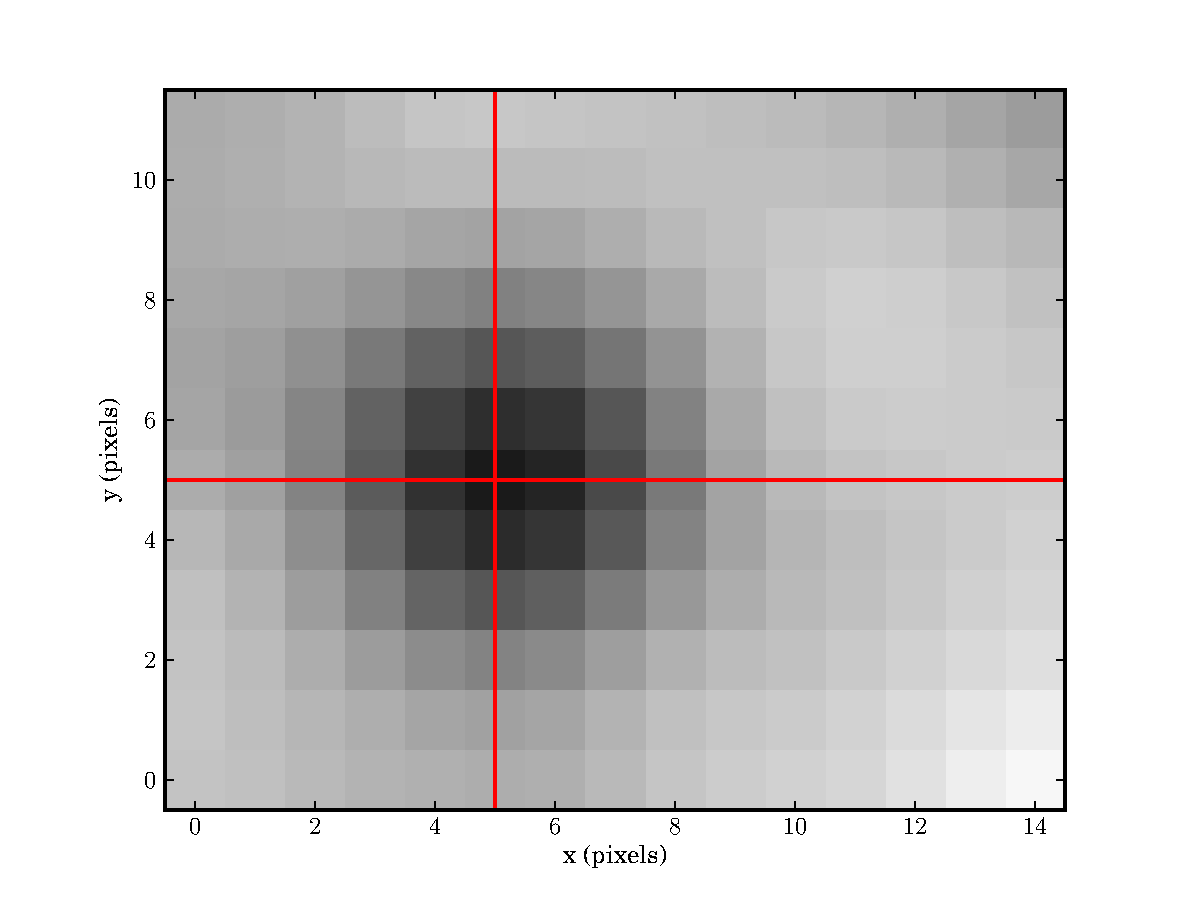
\includegraphics[width=0.3\textwidth]{f03a-bw}
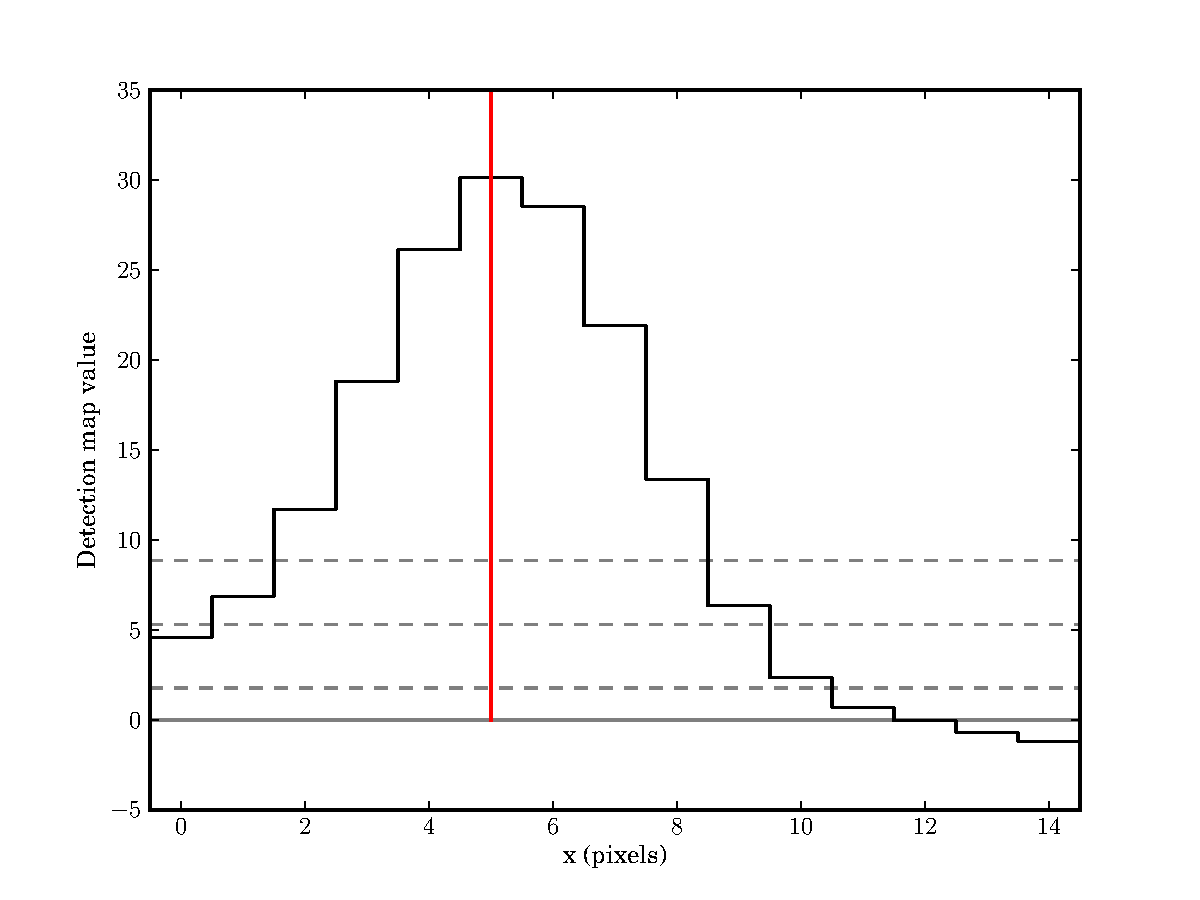
\includegraphics[width=0.3\textwidth]{f03b-bw} \\
  % ideal
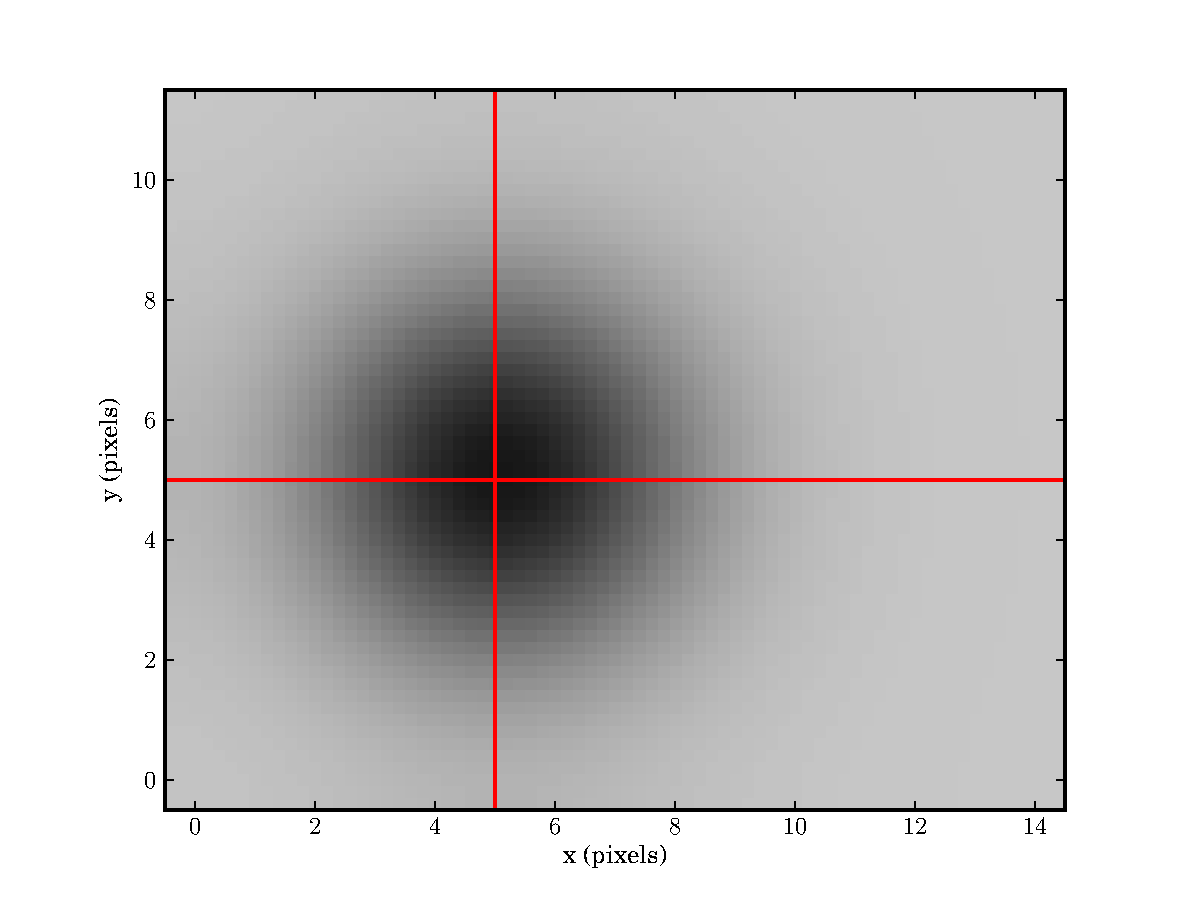
\includegraphics[width=0.3\textwidth]{f04c-bw}
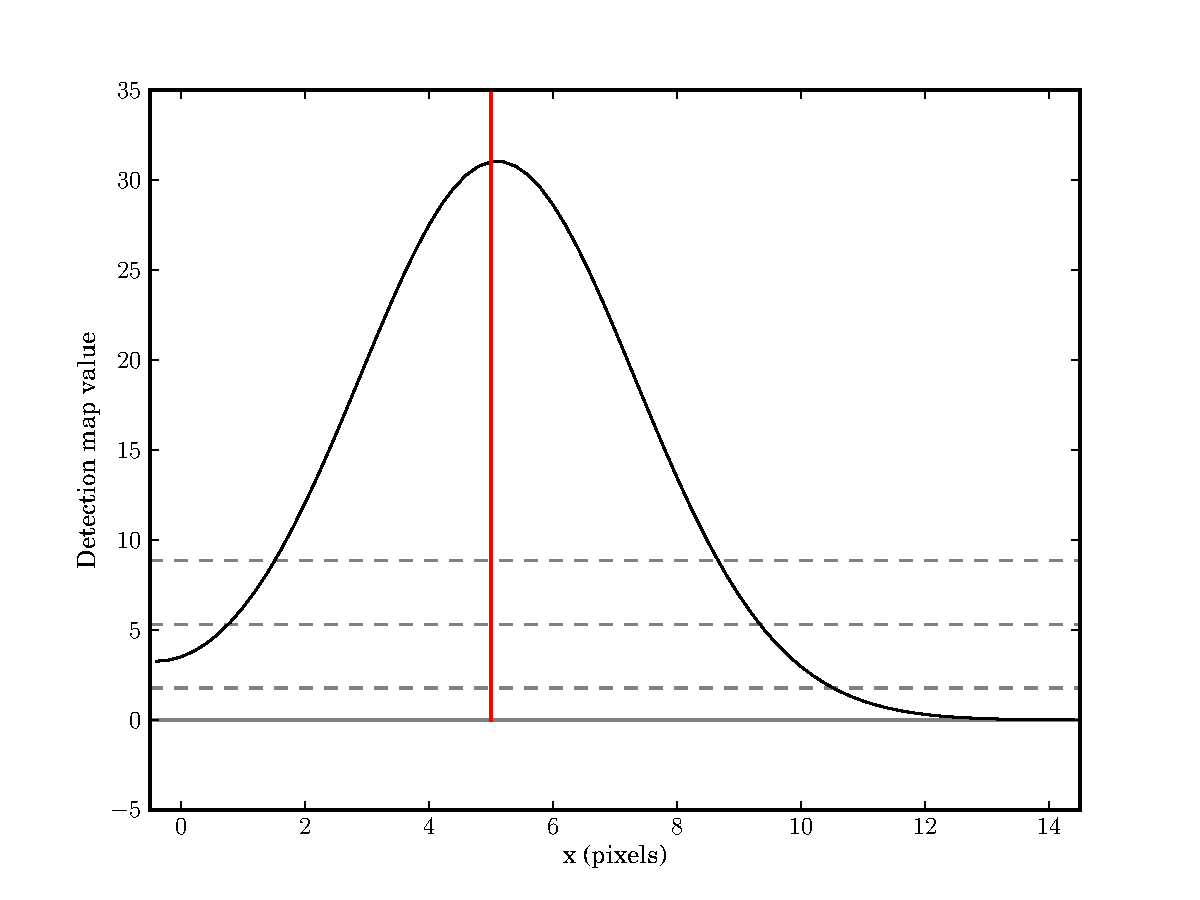
\includegraphics[width=0.3\textwidth]{f04d-bw} \\
% noisy
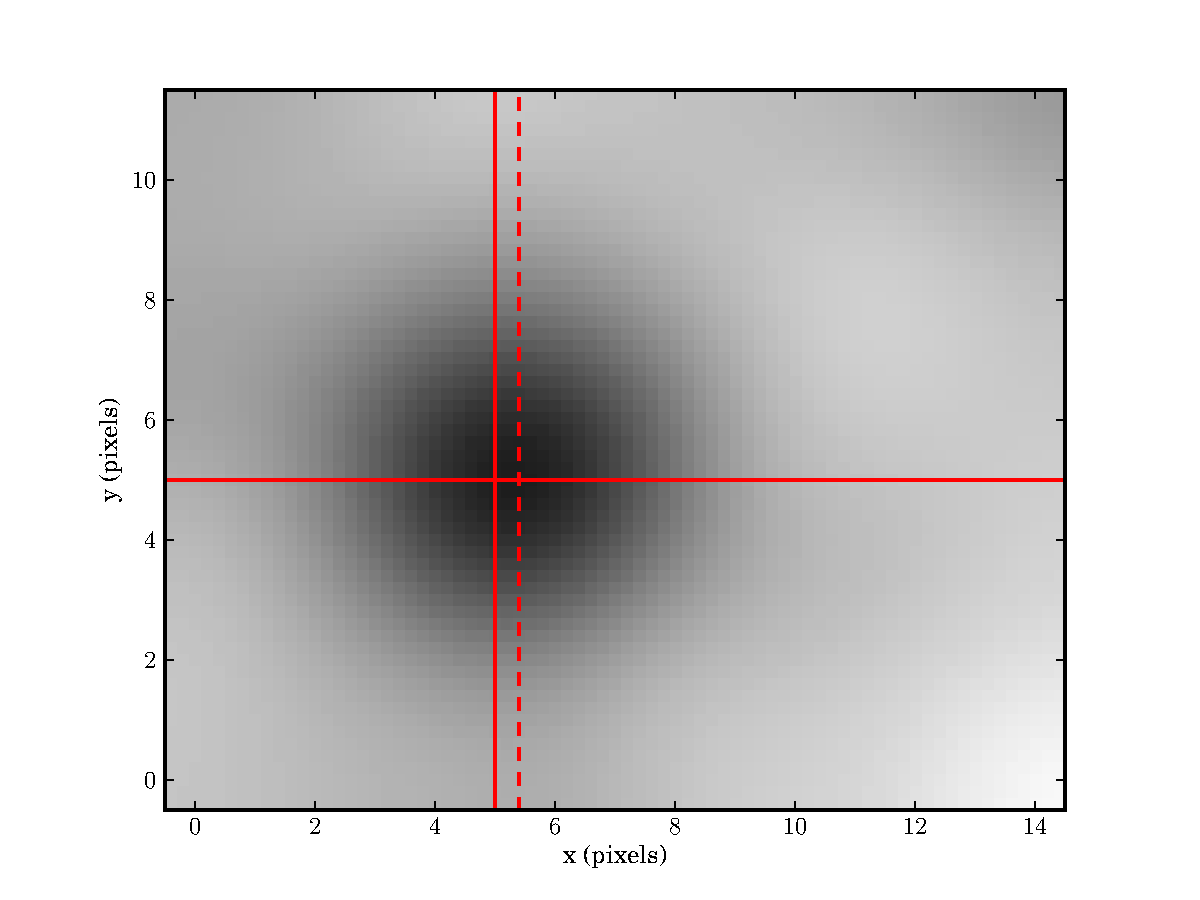
\includegraphics[width=0.3\textwidth]{f04a-bw}
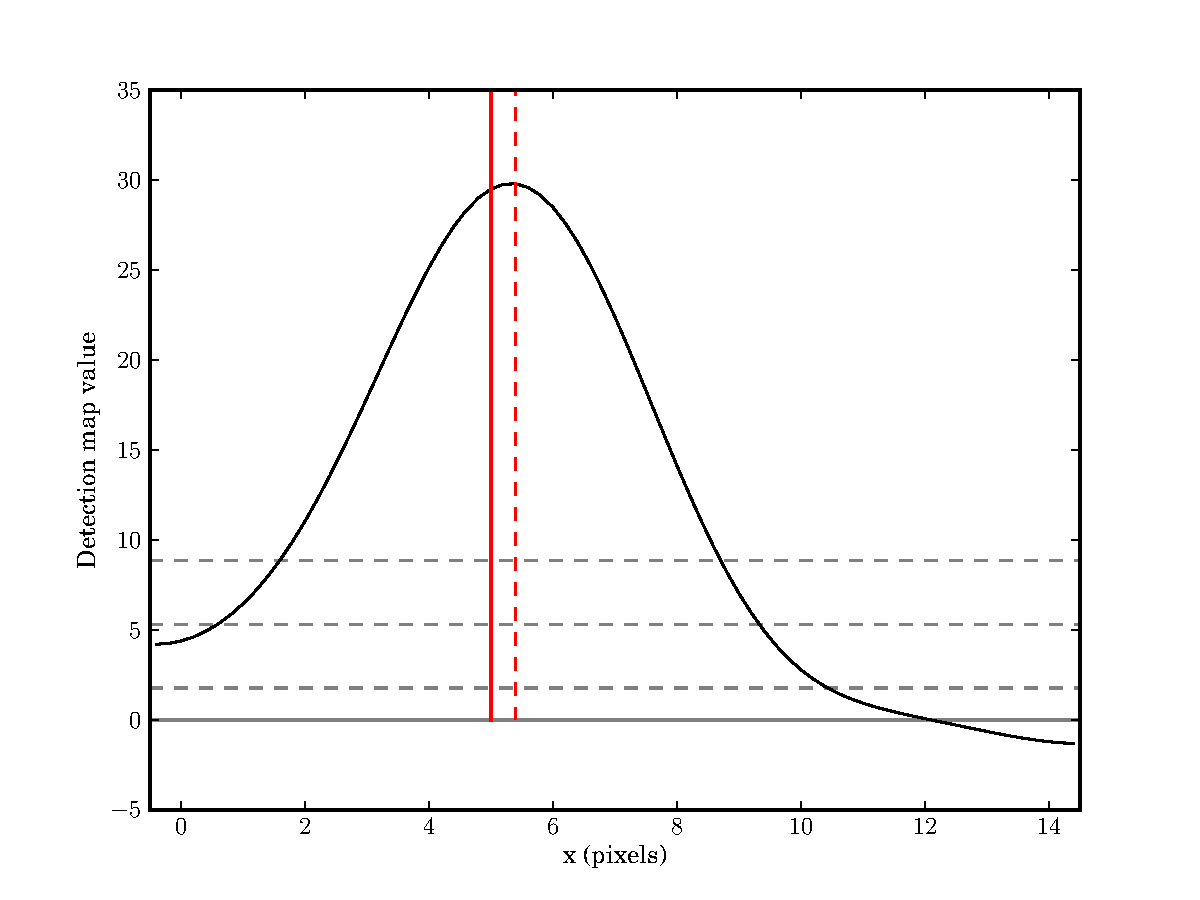
\includegraphics[width=0.3\textwidth]{f04b-bw}
\end{center}
\caption{The detection map of the example image.  \figpart{Top-left:}
  pixelized detection map.  \figpart{Top-right:} slice through $y=5$,
  with dashed lines showing $1$, $3$, and $5$ standard deviations of
  the noise in the detection map pixels.  \figpart{Bottom-left:}
  subsampled detection map. The true peak position is marked with
  solid lines.  The detected peak position is marked with dashed
  lines.  \figpart{Bottom-right:} slice through $y=5$.
\label{fig:detmap}}
\end{figure}

\begin{figure}
\begin{center}
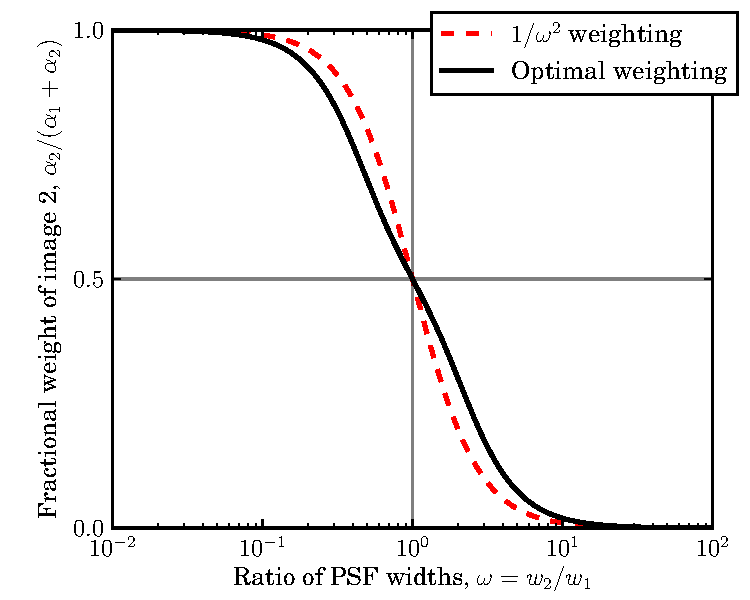
\includegraphics[width=0.49\textwidth]{coadd-weight-1}
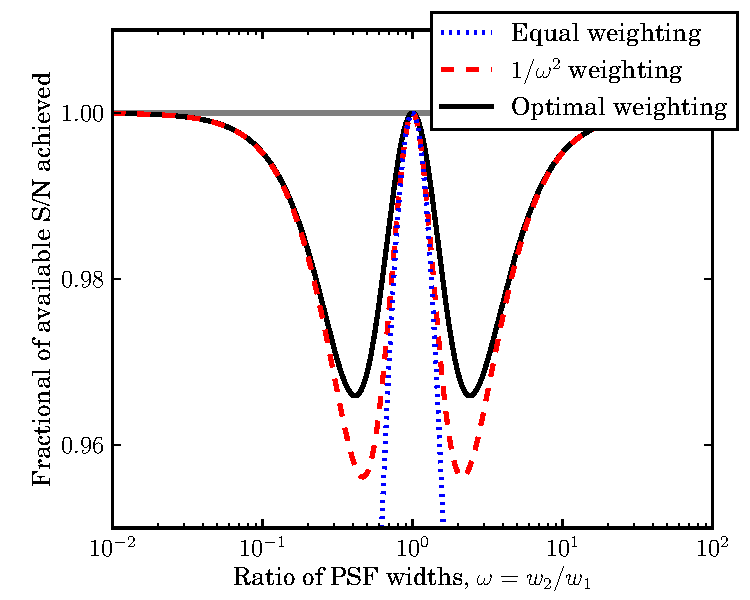
\includegraphics[width=0.49\textwidth]{coadd-weight-2}
\end{center}
\caption{\figpart{Left:} The fractional weight assigned to one image
  in an optimal co-add of two images with different PSF widths, from
  \eqnref{eq:coaddwt1}.  In the limit that image $I_2$ has a PSF that
  is much narrower ($\omega \ll 1$), the coadd weights that image
  highly.  When the PSF widths are equal ($\omega = 1$), the two
  images are assigned equal weight, and when the PSF is much broader
  ($\omega \gg 1$) the weight goes to zero, as expected.  Also shown is
  the weighting by $1/\omega^2$, which has a similar overall shape.
  \figpart{Right:} The fraction of the available signal-to-noise
  captured by the $1/\omega^2$ and optimal coadd weightings.  Notice
  that neither captures all the available signal-to-noise when the
  PSFs are different, since detecting sources in a coadd necessarily
  entails using a ``mismatched filter'' rather than an optimal
  ``matched filter'' for detection.  Using the optimal coadd weighting
  achieves about a $1\%$ increase in signal-to-noise in detecting
  point sources when the PSF widths differ by a factor of two.
  \label{fig:coaddwt1}}
\end{figure}




\end{document}

